\setchapterimage[8cm]{Paul Pastourmatzis Unsplash}
\setchapterpreamble[u]{\margintoc}
\chapter{常微分方程}
\labch{ode}

本章主要是《常微分方程》王高雄(第三版)的笔记整理.

\section{一阶线性微分方程}

\subsection{分离变量法的应用}

分离变量法,对于 $\displaystyle \frac{dy}{dx}=f(x,y)$ 类型,注意可能的 $\displaystyle y=\text{Const.}$ 的解.

注意 $\displaystyle \frac{dy}{y}=d\ln \lvert y \rvert$.

变量代换,对于 $\displaystyle \frac{dy}{dx}=f\left( \frac{y}{x} \right)$,换元 $\displaystyle u=\frac{y}{x}$,于是 $\displaystyle x=uy$,就可以变成可分离变量的形式.

注意 $\displaystyle \int \cot x=\ln \lvert \sin x \rvert,\int \tan x=-\ln \lvert \cos x \rvert$.
$$
    \frac{dy}{dx}=-\frac{e^{ y^{2}+3x }}{y}\Rightarrow-\frac{y}{e^{ y^{2} }}dy=e^{ 3x }dx\Rightarrow\frac{1}{2}e^{ -y^{2} }=\frac{1}{3}e^{ 3x }+\text{Const.}
$$
对于 $\displaystyle \frac{dy}{dx}=\frac{2x-y+1}{x-2y+1}$,先求解
$$
    \left\{\begin{array}{l}
        2x-y+1=0 \\
        x-2y+1=0
    \end{array}\right.
$$
得到 $\displaystyle x=-\frac{1}{3},y=\frac{1}{3}$. 变量代换令 $\displaystyle x=X-\frac{1}{3},y=Y+\frac{1}{3}$,目的是变成齐次微分方程,再令 $\displaystyle u=\frac{Y}{X}$,即可.

思路就是强行换元分离变量,直到化为可分离变量的形式.
$$
    \frac{dy}{dx}=\frac{y^{6}-2x^{2}}{2xy^{5}+x^{2}y^{2}}\Rightarrow\frac{y^{2}dy}{dx}=\frac{(y^{3})^{2}-2x^{2}}{2xy^{3}+x^{2}}\overset{ u=y^{3} }{ \Rightarrow }\frac{1}{3}\frac{du}{dx}=\frac{u^{2}-2x^{2}}{2xu+x^{2}}=\frac{1-2\left( \frac{u}{x} \right)^{2}}{2\frac{u}{x}+1}
$$
对于 $\displaystyle \frac{x}{y}\frac{dy}{dx}=f(xy)$,可以换元 $\displaystyle xy=u$,变成变量分离方程 $\displaystyle \frac{du}{dx}=\frac{u(f(u)+1)}{x}$. 比如
$$
    x(1+x^{2}y^{2})dx=xdy
$$
对于具有性质 $\displaystyle x(t+s)=\frac{x(t)+x(s)}{1-x(t)x(s)}$ 的函数,先带入 $\displaystyle s=t=0$,再带入 $\displaystyle x'(t)=\lim_{ s \to 0 }\frac{x(t+s)-x(t)}{s}$ 中.

对于\textbf{伯努利微分方程} $\displaystyle \frac{dy}{dx}=P(x)y+Q(x)y^{n}$,其中 $\displaystyle n\neq0,1$,只需要两边乘上 $\displaystyle y^{-n}$,就可以得到
$$
    y^{-n}\frac{dy}{dx}=(1-n)^{-1}\frac{dy^{1-n}}{dx}=P(x)y^{1-n}+Q(x)
$$
换元令 $\displaystyle z=y^{1-n}$ 就有标准形式,再利用常数变易法就可以得到结果.

\subsection{积分因子法}

完整的积分因子法:\href{https://math.libretexts.org/Courses/Mount_Royal_University/MATH_2200%3A_Calculus_for_Scientists_II/Appendix/A1%3A_Introduction_to_Differential_Equations/3.8%3A_Integrating_Factors}{Integrating Factors}

当微分方程 $\displaystyle P(x,y)dx+Q(x,y)dy=0$ 是\textbf{恰当微分方程}时,即有 $\displaystyle \frac{ \partial P }{ \partial y }=\frac{ \partial Q }{ \partial x }$,这个时候对于方程的解 $\displaystyle u(x,y)$,有 $\displaystyle \frac{ \partial u }{ \partial y }=P,\frac{ \partial u }{ \partial x }=Q$,于是积分得到 $\displaystyle u=\int P(x,y)dy+\phi(x)$,带回 $\displaystyle \frac{ \partial u }{ \partial x }=Q$ 解得 $\displaystyle \phi(x)$,就有了方程的解.

但是有时候微分方程不是恰当微分方程,即 $\displaystyle \frac{ \partial P }{ \partial y }-\frac{ \partial Q }{ \partial x }\neq0$,这时候要引入积分因子 $\displaystyle \mu=\mu(x,y)$,凑出恰当微分方程 $\displaystyle \mu Pdx+\mu Qdy=0$. 即有 $\displaystyle \frac{ \partial \mu P }{ \partial y }=\frac{ \partial \mu Q }{ \partial x }$,即 $\displaystyle Q\frac{ \partial \mu }{ \partial x }-P\frac{ \partial \mu  }{ \partial y }=\left( \frac{ \partial P }{ \partial y }-\frac{ \partial Q }{ \partial x } \right)\mu$. 我们希望 $\displaystyle \mu$ 只与一个变量有关,这样便于计算出 $\displaystyle \mu$,以 $x$ 为例,$\displaystyle \mu$ 只与 $x$ 有关的充要条件是 $\displaystyle \frac{\frac{ \partial P }{ \partial y }-\frac{ \partial Q }{ \partial x }}{Q}=\psi(x)$,于是解出 $\displaystyle \mu=e^{ \int \psi(x) \, dx }$. 同理,$\displaystyle \mu$ 只与 $\displaystyle y$ 有关的充要条件为 $\displaystyle \displaystyle \frac{\frac{ \partial P }{ \partial y }-\frac{ \partial Q }{ \partial x }}{-P}=\phi(y)$,解得 $\displaystyle \mu=e^{ \int \phi(y) \, dy }$.

\begin{exercise}
    对于齐次微分方程\sidenote{形如 $\frac{d y}{d x}=f\left(\frac{y}{x}\right)$ 的一阶微分方程称为齐次微分方程,如 $\displaystyle dy=\frac{x^{2}+y^{2}}{xy}dx$.} $\displaystyle P(x,y)dx+Q(x,y)dy=0$,若 $\displaystyle xP+yQ\neq0$,则有积分因子 $\displaystyle \mu=\frac{1}{xP+yQ}$.
\end{exercise}

\subsubsection{求解一般的\texorpdfstring{$\mu(x,y)$}{mu(x,y)}}

考虑齐次微分方程
\begin{equation}\label{eq:integrating_factor}
    M(x,y)dx+N(x,y)dy=0
\end{equation}

\begin{theorem}\label{thm:integrating_factor}
    令 $M,N,M_y,N_y$ 在开矩形 $R$ 上连续,那么
    \begin{enumerate}
        \item 如果 $(M_y-N_x)/N$ 在 $R$ 上与 $y$ 无关,那么定义
              $$p(x)=\frac{M_y-N_x}{N}$$
              则方程\ref{eq:integrating_factor} 有积分因子
              \begin{equation}\label{eq:integrating_factor_1}
                  \mu(x)=\pm \exp\left( \int p(x) \, dx \right)
              \end{equation}
        \item 如果 $(N_x-M_y)/M$ 在 $R$ 上与 $x$ 无关,那么定义
              $$q(y)=\frac{N_x-M_y}{M}$$
              则方程\ref{eq:integrating_factor} 有积分因子
              \begin{equation}\label{eq:integrating_factor_2}
                  \mu(y)=\pm \exp\left( \int q(y) \, dy \right)
              \end{equation}
    \end{enumerate}
\end{theorem}

一般而言,我们希望积分因子有形式 $\mu(x,y)=P(x)Q(y)$,这样便于计算. \sidenote[][2mm]{这样就有
    \begin{align*}
        \mu_x(x,y) & =P'(x)Q(y), \\
        \mu_y(x,y) & =P(x)Q'(y).
    \end{align*}
}

带入式子 $\displaystyle \frac{ \partial (\mu M) }{ \partial y }=\frac{ \partial (\mu N) }{ \partial x }$,得到
\begin{equation}\label{eq:integrating_factor_3}
    M(x) N(y)\left(M_y-N_x\right)=M'(x) N(y) N-M(x) N'(y) M,
\end{equation}
令 $p(x)=P'(x)/P(x)$,$q(y)=Q'(y)/Q(y)$,则有
\begin{equation}\label{eq:integrating_factor_4}
    M_y-N_x=p(x)N-q(y)M.
\end{equation}
\marginnote{意思就是只要把 $M_y-N_x$ 写成 $p(x)N-q(y)M$ 的形式,就可以找到积分因子.}
于是我们反解出
\begin{equation}\label{eq:integrating_factor_5}
    P(x)=\pm \exp\left( \int p(x) \, dx \right)\qquad Q(y)=\pm\exp\left( \int q(y) \, dy \right).
\end{equation}
积分因子为 $\mu(x,y)=P(x)Q(y)$.\sidenote[][2mm]{没有一般的方法说明满足方程\ref{eq:integrating_factor_4} 的 $p(x)$ 和 $q(y)$ 是否存在.}

\begin{exercise}
    求如下方程的积分因子:
    \begin{equation}\label{eq:integrating_factor_6}
        2x y^3 dx+(3x^2y^2+x^2y^3+1)dy=0. \marginnote{这不是恰当微分方程.}
    \end{equation}
\end{exercise}

\begin{solution}
    在方程\ref{eq:integrating_factor_6} 中,$M=2xy^3$,$N=3x^2y^2+x^2y^3+1$,于是
    \begin{align*}
        M_y-N_x=6xy^2-(6xy^2+2xy^3)=-2xy^3=-M,
    \end{align*}
    根据定理\ref{thm:integrating_factor},可以找到与$x$无关的积分因子,记$q(y)=1$,因为
    \begin{equation*}
        \int q(y) \, dy=\int 1 \, dy=y,
    \end{equation*}
    所以$\mu(y)=e^y$ 是一个积分因子,于是得到恰当微分方程
    \begin{equation*}
        2xy^3e^ydx+(3x^2y^2+x^2y^3+1)e^ydy=0.
    \end{equation*}
    于是
    \begin{align}
        F_x(x,y) & =2xy^3e^y,\label{eq:integrating_factor_7}                 \\
        F_y(x,y) & =3x^2y^2e^y+x^2y^3e^y+e^y.\label{eq:integrating_factor_8}
    \end{align}
    对方程\ref{eq:integrating_factor_7} 关于$x$积分得到
    \begin{equation*}
        F(x,y)=x^2y^3e^y+\phi(y).
    \end{equation*}
    关于$y$求导得到
    \begin{equation*}
        F_y(x,y)=3x^2y^2e^y+x^2y^3e^y+e^y=\frac{d\phi(y)}{dy}.
    \end{equation*}
    与方程\ref{eq:integrating_factor_8} 比较得到 $\phi '(y)=e^y$,于是 $\phi(y)=e^y$,于是微分方程\ref{eq:integrating_factor_6}的解为
    \begin{equation*}
        (x^2y^3+1)e^y=c.\marginnote{这是一个隐式解.}
    \end{equation*}
\end{solution}

\subsection{一阶隐式微分方程与解的参数表示}

\begin{example}
    求解方程 $\displaystyle xy'^{3}=1+y'$
\end{example}

\begin{solution}
    $$
        xy'^{3}=1+y'\overset{ p=y' }{ \Rightarrow } x=\frac{1}{p^{3}}+\frac{1}{p^{2}}
    $$
    两边对 $y$ 求导得到
    $$
        \frac{1}{p}=\left( -\frac{3}{p^{4}} -\frac{2}{p^{3}}  \right)\frac{dp}{dy}\Rightarrow dy=\left( -\frac{3}{p^{3}} -\frac{2}{p^{2}}  \right)dp\Rightarrow y=\frac{3}{2p^{2}}+\frac{2}{p}+c
    $$
    故原方程的通解为
    $$
        \left\{\begin{array}{l}
            x=\frac{1}{p^{3}}+\frac{1}{p^{2}} \\
            y=\frac{3}{2p^{2}} +\frac{2}{p}+c
        \end{array}\right.
    $$
    $p$ 为参数且 $\displaystyle p\neq0$,$c$ 为任意常数.
\end{solution}

\begin{note}
    不显含$x$或$y$的微分方程。解是参数形式
    \[
        x=x(t),y=y(t)
    \]
\end{note}
\subsubsection{不显含$x$的微分方程}

\begin{example}
    求解方程 $x^3+y^{\prime 3}-3 x y^{\prime}=0\left(\right.$ 这里 $\left.y^{\prime}=\frac{\mathrm{d} y}{\mathrm{~d} x}\right)$.
\end{example}

\begin{solution}
    令 $y^{\prime}=p=t x$,则由方程得
    $$
        x=\frac{3 t}{1+t^3},
    $$
    从而
    $$
        p=\frac{3 t^2}{1+t^3}
    $$
    于是
    $$
        \mathrm{d} y=\frac{9\left(1-2 t^3\right) t^2}{\left(1+t^3\right)^3} \mathrm{~d} t
    $$
    积分之,得到
    $$
        y=\int \frac{9\left(1-2 t^3\right) t^2}{\left(1+t^3\right)^3} \mathrm{~d} t=\frac{3}{2} \frac{1+4 t^3}{\left(1+t^3\right)^2}+c
    $$
    因此,方程的通解表成参数形式
    $$
        \left\{\begin{array}{l}
            x=\frac{3 t}{1+t^3}, \\
            y=\frac{3}{2} \frac{1+4 t^3}{\left(1+t^3\right)^2}+c
        \end{array}\right.
    $$
\end{solution}

\subsubsection{不显含$y$的微分方程}

\begin{example}
    例 5 求解方程 $y^2\left(1-y^{\prime}\right)=\left(2-y^{\prime}\right)^2$.
\end{example}

\begin{solution}
    令 $2-y^{\prime}=y t$ ,则与原微分方程消去 $y^{\prime}$ 后,有
    $$
        y^2(y t-1)=y^2 t^2,
    $$
    由此得
    $$
        y=\frac{1}{t}+t
    $$
    并且
    $$
        y^{\prime}=1-t^2,
    $$
    这是原微分方程的参数形式. 因此
    $$
        \mathrm{d} x=\frac{\mathrm{d} y}{y}=-\frac{1}{t^2} \mathrm{~d} t,
    $$
    积分之,得到
    $$
        x=\frac{1}{t}+c
    $$
    于是求得方程的参数形式的通解为
    $$
        \left\{\begin{array}{l}
            x=\frac{1}{t}+c, \\
            y=\frac{1}{t}+t
        \end{array}\right.
    $$
    或者消去参数 $t$ 得
    $$
        y=x+\frac{1}{x-c}-c,
    $$
    其中 $c$ 为任意常数.
    此外,当 $y^{\prime}=0$ 时原方程变为 $y^2=4$ ,于是 $y= \pm 2$ 也是方程的解.
\end{solution}


\section{存在唯一性理论}

\subsection{构造Picard序列求近似解}

\begin{note}
    以操作主义视之,对于微分方程,$\displaystyle y'=f(x,y)$,先求出平凡解 $\displaystyle \varphi_{0}$,再利用算子 $\displaystyle A(\varphi)(x)=y_{0}+\int_{x_{0}}^{x} f(\xi,\varphi(\xi)) \, d\xi$. 构造 Picard 序列,求出 $\displaystyle \varphi_{1},\varphi_{2},\dots$
\end{note}

\subsubsection{误差估计}

$\displaystyle f(x,y)$ 在矩形区域 $\displaystyle R:[x_{0}-a,x_{0}+a]\times[y_{0}-b,y_{0}+b]$ 上满足 Lipschitz 条件,即存在常数 $\displaystyle L>0$,使得 $\displaystyle \lvert f(x,y_{1})-f(x,y_{2}) \rvert\leq L\lvert y_{1}-y_{2} \rvert$ 对所有的 $\displaystyle (x, y_{1}), (x, y_{2})\in R$ 都成立.

记 $\displaystyle M=\max_{(x,y)\in R}\lvert f(x,y) \rvert,h=\min\left( a,\frac{b}{M} \right)$. 于是解 $\displaystyle y=\varphi(x)$ 在区间\sidenote[][2mm]{这是\textbf{解的存在区间}的定义.} $\displaystyle [x_{0}-h,x_{0}+h]$ 上存在,且\textbf{误差估计}为
$$
    \left|\varphi_n(x)-\varphi(x)\right| \leqslant \frac{M L^n}{(n+1)!} h^{n+1}
$$
\begin{note}
    解的存在唯一性可以用压缩映射定理证明\cite{Arnold},并延拓到 $\displaystyle [x_{0}-h,x_{0}+h]$ 上.
\end{note}

\subsection{解对初值与参数的依赖性}

之前我们把初值 $\displaystyle (t_{0},x_{0})$ 看为固定的,得到的解 $\displaystyle \varphi$ 只是 $\displaystyle t$ 的函数,如果初值条件发生了改变,则相应的解也会改变,为了研究解对初值改变的稳定性,我们将解视为 $\displaystyle \varphi(t,t_{0},x_{0})$. 如果方程中还包含参数 $\displaystyle \lambda$,那就视为 $\displaystyle \varphi(t,t_{0},x_{0},\lambda)$. 我们有必要研究解 $\displaystyle \varphi(t,t_{0},x_{0},\lambda)$ 的连续依赖性和可微依赖性. 一般地,可以不妨设初值条件为 $\displaystyle \mathbf{x}(0)=0$,否则平移变换. 于是我们研究如下的微分方程初值问题:
$$
    \frac{d\mathbf{x}}{dt}=\mathbf{f}(t,\mathbf{x},\lambda)\qquad \mathbf{x}(0)=0
$$
\begin{note}
    如果函数 $f$ 满足 Lipschitz 条件,则解 $\displaystyle \varphi(t,t_{0},x_{0},\lambda)$ 对初值 $\displaystyle (t_{0},x_{0})$ 连续依赖,对参数 $\displaystyle \lambda$ 可微.
\end{note}
接下来研究对于参数的求导性质:

对于初值问题
\begin{equation}\label{dhak}
    \frac{\mathrm{d} \boldsymbol{x}}{\mathrm{~d} t}=\boldsymbol{f}(t, \boldsymbol{x}, \boldsymbol{\lambda}), \quad \boldsymbol{x}\left(0\right)=\boldsymbol{0}_0
\end{equation}
\begin{corollary}
    $z:=\frac{\partial \varphi}{\partial t_0}$ 满足初值问题
    \begin{equation}\label{eq:ode_1}
        \frac{\mathrm{d} z}{\mathrm{~d} t}=\left(\frac{\partial}{\partial x} f(t, \varphi, \lambda)\right) z, \quad z\left(t_0\right)=-f\left(t_0, x_0, \lambda\right)
    \end{equation}
    $z:=\frac{\partial \varphi}{\partial x_0}$ 满足初值问题
    \begin{equation}\label{eq:ode_2}
        \frac{\mathrm{d} z}{\mathrm{~d} t}=\left(\frac{\partial}{\partial x} f(t, \varphi, \lambda)\right) z, \quad z\left(t_0\right)=1
    \end{equation}
    $z:=\frac{\partial \varphi}{\partial \lambda}$ 满足初值问题
    \begin{equation}\label{eq:ode_3}
        \frac{\mathrm{d} z}{\mathrm{~d} t}=\left(\frac{\partial}{\partial x} f(t, \varphi, \lambda)\right) z+\frac{\partial}{\partial \lambda} f(t, \varphi, \lambda), \quad z\left(t_0\right)=0
    \end{equation}
\end{corollary}
\begin{note}
    上述三个线性方程(\ref{eq:ode_1})、(\ref{eq:ode_2})、(\ref{eq:ode_3})称为初值问题\ref{dhak}关于 $t_0$ , $x_0, \lambda$ 的线性变分方程. 证明是利用初值问题\ref{dhak}的等价积分方程来对 $t_0, x_0$, $\lambda$ 作相应的求导.
\end{note}

对于
$$
    \varphi(t,t_{0},x_{0},\lambda)=x_{0}+\int_{t_{0}}^{t} f(\tau,\varphi(\tau,t_{0},x_{0},\lambda),\lambda) \, d\tau \qquad \varphi(t_{0},t_{0},x_{0},\lambda)=x_{0}
$$
考虑作用 $\displaystyle \frac{ \partial   }{ \partial x_{0} }$ 得到
$$
    \frac{ \partial \varphi }{ \partial x_{0} } (t,t_{0},x_{0},\lambda)=1+\int_{t_{0}}^{t} \frac{ \partial f }{ \partial x } (\tau,\varphi(\tau,t_{0},x_{0},\lambda),\lambda)\cdot \frac{ \partial \varphi }{ \partial x_{0} } (\tau,\varphi(\tau,t_{0},x_{0},\lambda),\lambda) \, d\tau
$$
于是解为
$$
    \frac{d}{dt}\frac{ \partial \varphi }{ \partial x_{0} } =\frac{ \partial f }{ \partial x } (t,\varphi(t,t_{0},x_{0},\lambda),\lambda)\cdot \frac{ \partial \varphi }{ \partial x_{0} } (t,\varphi(t,t_{0},x_{0},\lambda),\lambda)
$$
初值条件为
$$
    \frac{ \partial \varphi }{ \partial x_{0} } (t_{0},t_{0},x_{0},\lambda)=1.
$$
考虑作用 $\displaystyle \frac{ \partial   }{ \partial \lambda }$ 得到
{\small $$
    \frac{ \partial \varphi }{ \partial \lambda } (t,t_{0},x_{0},\lambda)=0+\int_{t_{0}}^{t} \frac{ \partial f }{ \partial x } (\tau,\varphi(\tau,t_{0},x_{0},\lambda),\lambda)\cdot \frac{ \partial \varphi }{ \partial \lambda } (\tau,t_{0},x_{0},\lambda)+\frac{ \partial f }{ \partial \lambda } (\tau,\varphi(\tau,t_{0},x_{0},\lambda),\lambda) \, d\tau
$$}
于是解为
$$
    \frac{d}{dt}\frac{ \partial f }{ \partial \lambda } (t,t_{0},x_{0},\lambda)=\frac{ \partial f }{ \partial x } (t,\varphi(t,t_{0},x_{0},\lambda),\lambda)\cdot \frac{ \partial \varphi }{ \partial \lambda } (t,t_{0},x_{0},\lambda)+\frac{ \partial f }{ \partial \lambda } (t,\varphi(t,t_{0},x_{0},\lambda),\lambda)
$$
初值条件为
$$
    \frac{ \partial f }{ \partial \lambda } (t_{0},t_{0},x_{0},\lambda)=0
$$

\subsection{求奇解}

以下将介绍如何求解参数曲线族的包络和微分方程的奇解.

求解参数曲线组的包络关键在于对参数求导后消去参数,还要画图判断是否为包络.

对于一族直线:$\displaystyle x\cos\alpha+y\sin\alpha-p=0$,其中 $\displaystyle \alpha$ 是参数, $p$ 是常数.

对 $\displaystyle \alpha$ 求导得到 $\displaystyle -x\sin\alpha+y\cos\alpha=0$,自然地消掉 $\displaystyle \alpha$ 得到 $\displaystyle x^{2}+y^{2}=p^{2}$ 为该族直线的包络.

对于曲线族 $\displaystyle (y-c)^{2}-\frac{2}{3}(x-c)^{3}=0$,其中 $c$ 是参数.

对 $\displaystyle c$ 求导得到 $\displaystyle -2(y-c)+2(x-c)^{2}=0$,自然消参得到 $\displaystyle (x-c)^{3}\left[ (x-c)-\frac{2}{3} \right]=0$,解得 $\displaystyle y=x$ 或 $\displaystyle y=x-\frac{2}{9}$. 然而从图像上看前者不是包络,而后者是包络.

\subsubsection{求奇解}

由奇解的定义容易知道一阶微分方程的通解的包络 (如果存在) 一定是奇解;反之,微分方程的奇解 (如果存在) 也是微分方程的通解的包络.

\begin{note}

    微分方程的通解指的不是全部解.
\end{note}
为了求出奇解,可以先求出微分方程的通解,然后求通解的包络.

接下来介绍另一种求奇解的方法.

由隐函数定理知道,如果 $\displaystyle F(x,y,y')=0$ 关于 $\displaystyle x,y,y'$ 连续可微,则只要 $\displaystyle \frac{ \partial F }{ \partial y' }\neq0$ 就能保证解的唯一性,因此奇解 (如果存在) 必须同时满足下列方程
$$
    F(x,y,y')=0\qquad \frac{ \partial F(x,y,y') }{ \partial y' } =0.
$$
于是方程 $\displaystyle F(x,y,y')=0$ 的奇解包含在如下方程组消去 $p$ 而得到的曲线中
$$
    \left\{\begin{array}{l}
        F(x,y,p)=0 \\
        \frac{ \partial F }{ \partial p } (x,y,p)=0
    \end{array}\right.
$$
该曲线称为方程 $\displaystyle F(x,y,y')=0$ 的 $p$ -\textbf{判别曲线}. $\displaystyle p$ -判别曲线是否是方程的奇解,需要进一步检验.

\paragraph{Example}

\begin{example}
    求方程 $\displaystyle y'^{2}+y^{2}-1=0$ 的奇解
\end{example}

考虑 $p$ -判别曲线:
$$
    \left\{\begin{array}{l}
        p^{2}+y^{2}-1=0 \\
        2p=0
    \end{array}\right.
$$
消去 $p$ 得到 $p$ -判别曲线为 $\displaystyle y=\pm1$. 容易验证,这两条直线都是方程的奇解,因为原方程的通解为 $\displaystyle y=\sin(x+c)$.

\begin{example}
    求方程 $\displaystyle y=2x\frac{dy}{dx}-\left( \frac{dy}{dx} \right)^{2}$ 的奇解
\end{example}

求得 $p$ -判别曲线为 $\displaystyle y=x^{2}$,但是 $\displaystyle y=x^{2}$ 不是方程的解,故此方程没有奇解.

\subsubsection{克莱罗微分方程}
$$
    y=xp+f(p)\qquad \text{其中 }p=\frac{dy}{dx},f(p)\text{是 }p\text{ 的连续可微函数}
$$
其通解为直线族
$$
    y=cx+f(c)\qquad \text{其中 }c\text{ 为参数}
$$
其奇解就是该直线族的包络.

\section{高阶微分方程}

\subsection{高阶线性微分方程理论}

考虑如下的 $n$ 阶线性微分方程;
\begin{equation}\label{4.1}
    x^{(n)}+a_{1}(t)x^{(n-1)}+\dots+a_{n-1}(t)x+a_{n}(t)x=f(t)
\end{equation}
其中 $\displaystyle a_{i}(t)$ 和 $\displaystyle f(t)$ 都是区间 $\displaystyle t\in[a,b]$ 上的连续函数. 如果 $\displaystyle f(t)\equiv0$,则方程 式\ref{4.1} 变为
\begin{equation}\label{4.2}
    x^{(n)}+a_{1}(t)x^{(n-1)}+\dots+a_{n-1}(t)x+a_{n}(t)x=0
\end{equation}
这被称为 $n$ 阶齐次线性微分方程,而 式\ref{4.1} 被称为 $n$ 阶非齐次线性微分方程.
\subsubsection{解法}

\paragraph{齐次线性微分方程}

直接猜出 $n$ 个解 $\displaystyle x_{1}(t),\dots,x_{n}(t)$,故通解为 $\displaystyle x(t)=c_{1}x_{1}(t)+\dots+c_{n}x_{n}(t)$,其中 $\displaystyle c_{i}$ 为参数.

\paragraph{非齐次线性微分方程}

\begin{note}
    使用常数变易法.
\end{note}
联立如下等式
$$
    \left\{\begin{array}{l}
        x_{1}^{(i)}(t)c_{1}'(t)+\dots+x_{n}^{(i)}(t)c_{n}'(t)=0 \qquad i=0,1,\dots,n-2 \\
        x_{1}^{(n-1)}(t)c_{1}'(t)+\dots+x_{n}^{(n-1)}(t)c_{n}'(t)=f(t)
    \end{array}\right.
$$
解出 $\displaystyle c_{i}'(t)=\varphi _{i}'(t),i=1,2,\dots,n$,积分得到 $\displaystyle c_{i}(t)=\int \varphi _{i}(t) \, dt+\gamma _{i}$,其中 $\displaystyle \gamma _{i}$ 是任意常数. 故通解为
$$
    x=\sum_{i=1}^{n} \gamma _{i}x_{i}(t)+\sum_{i=1}^{n} x_{i}(t)\int \varphi _{i}(t) \, dt
$$
\subparagraph{示例}

求方程 $\displaystyle x''+x=\frac{1}{\cos t}$ 的通解.

已知它的对应齐次线性微分方程的基本解组为 $\displaystyle \cos t,\sin t$. 应用常数变易法,令
$$
    x=c_{1}(t)\cos t+c_{2}(t)\sin t
$$
把它带入方程,则可得决定 $\displaystyle c_{1}'(t)$ 和 $\displaystyle c_{2}'(t)$ 的两个方程
$$
    \left\{\begin{array}{l}
        \cos t \cdot c_{1}'(t)+\sin t\cdot c_{2}'(t)=0 \\
        -\sin t\cdot c_{1}'(t)+\cos t\cdot c_{2}'(t)=\frac{1}{\cos t}
    \end{array}\right.
$$
解得
$$
    c_{1}'(t)=-\frac{\sin t}{\cos t},\qquad c_{2}'(t)=1
$$
由此
$$
    c_{1}(t)=\ln \lvert \cos t \rvert +\gamma_{1},\qquad c_{2}(t)=t+\gamma_{2}
$$
于是原方程的通解为
$$
    x=\gamma_{1}\cos t+\gamma_{2}\sin t+\cos t\cdot \ln \lvert \cos t \rvert +t\sin t
$$
其中 $\displaystyle \gamma_{1},\gamma_{2}$ 为任意常数.

\subsection{一般线性微分方程求解}

记
\begin{gather}
    \frac{d^{n}}{dt^{n}}x+a_{1}(t)\frac{d^{n-1}}{dt^{n-1}}x+\dots+a_{n}(t)x=f(t)\tag{4.1}  \\
    \frac{d^{n}}{dt^{n}}x+a_{1}(t)\frac{d^{n-1}}{dt^{n-1}}x+\dots+a_{n}(t)x=0 \tag{4.2}
\end{gather}
若 式\ref{4.2} 中 $\displaystyle a_{i}(t)$ 都是实值函数,如果 $\displaystyle x=z(t)=\varphi(t)+i\psi(t)$ 是 式\ref{4.2} 的复值解,那么 $\displaystyle \varphi(t),\psi(t),\bar{z}(t)$ 都是 式\ref{4.2} 的解.

若 $\displaystyle \frac{d^{n}}{dt^{n}}x+a_{1}(t)\frac{d^{n-1}}{dt^{n-1}}x+\dots+a_{n}(t)x=u(t)+iv(t)$ 有复值解 $\displaystyle x=U(t)+iV(t)$,这里 $\displaystyle a_{i}(t),u(t),v(t)$ 都是实值函数,那么这个解的实部 $\displaystyle U(t)$ 和虚部 $\displaystyle V(t)$ 分别是下面两个方程的解
\begin{gather}
    \frac{d^{n}}{dt^{n}}x+a_{1}(t)\frac{d^{n-1}}{dt^{n-1}}x+\dots+a_{n}(t)x=u(t) \\
    \frac{d^{n}}{dt^{n}}x+a_{1}(t)\frac{d^{n-1}}{dt^{n-1}}x+\dots+a_{n}(t)x=v(t)
\end{gather}
\begin{note}
    若 $\displaystyle \forall i,a_{i}(t)=a_{i}$ 为常数,操作主义视之
\end{note}
方程 式\ref{4.2} 的特征方程为 $\displaystyle \lambda^{n}+a_{1}\lambda^{n-1}+\dots+a_{n}=0$,特征方程的 $n$ 个根为 $\displaystyle \lambda_{1},\lambda_{2},\dots,\lambda _{n}$.

若没有重根,那么方程 式\ref{4.2} 的解为 $\displaystyle e^{ \lambda_{1}t },e^{ \lambda_{2}t },\dots,e^{ \lambda _{n}t }$.

若有重根,则对于 $m$ 重根 $\displaystyle \lambda$,它对应的 $m$ 个解为 $\displaystyle e^{ \lambda t },t e^{ \lambda t },\dots,t^{m-1}e^{ \lambda t }$.

\textbf{欧拉方程}
$$
    x^{n}\frac{d^{n}}{dx^{n}}y+a_{1}x^{n-1}\frac{d^{n-1}}{dx^{n-1}}y+\dots+a_{n-1}x\frac{d}{dx}y+a_{n}y=0
$$
只需要变量替换 $\displaystyle x=e^{ t }$,就有
\begin{equation}\label{4.30}
    \displaystyle \frac{d^{n}}{dt^{n}}y+b_{1}\frac{d^{n-1}}{dt^{n-1}}y+\dots+b_{n}y=0
\end{equation}
化为一般的常系数线性微分方程. 于是 $\displaystyle y$ 有形如 $\displaystyle e^{ \lambda t }$ 的解,故 $\displaystyle y$ 有形如 $\displaystyle x^{\lambda}$ 的解. 因此可以将 $\displaystyle x^{K}$ ($K$ 为某个变量) 带入欧拉方程直接得到 (不用换元) 式\ref{4.30} 对应的代数方程 (特征方程):
$$
    K(K-1)\dots(K-n+1)+a_{1}K(K-1)\dots(K-n+2)+\dots+a_{n}=0
$$
单根对应的解是类似的 $\displaystyle x^{\lambda_{1}},\dots,x^{\lambda _{n}}$,而对于重数为 $m$ 的根 $\displaystyle K_{0}$ 有解 $\displaystyle x^{K_{0}},x^{K_{0}}\ln \lvert x \rvert,\dots,x^{K_{0}}\ln ^{m-1}\lvert x \rvert$.

\paragraph{Example}

求解 $\displaystyle x^{2}\frac{d^{2}y}{dx^{2}}+3x\frac{dy}{dx}+5y=0$.

对应的特征方程为 $\displaystyle K^{2}+2K+5=0$,解得 $\displaystyle K=-1\pm2i$,故方程的通解为 $\displaystyle y=x^{-1}(c_{1}\cos(2\ln \lvert x \rvert)+c_2\sin(2\ln \lvert x \rvert))$,其中 $\displaystyle c_{1},c_{2}$ 是任意常数.

\subsubsection{非齐次线性微分方程·比较系数法与拉普拉斯变换法}

\begin{note}
    当然可以利用\textbf{常数变易法}来做,但是往往太复杂,下面介绍当 $\displaystyle f(t)$ 具有某些特殊形状时所适用的一些方法——\textbf{比较系数法}和\textbf{拉普拉斯变换法},它们的特点时不用积分而是使用代数方法即可求解非齐次线性微分方程的特解.
\end{note}
\paragraph{比较系数法}

设 $\displaystyle f(t)=(b_{0}t^{m}+b_{1}t^{m-1}+\dots+b_{m})e^{ \lambda t }$,其中 $\displaystyle \lambda$ 及 $\displaystyle b_{i}\ (i=0,1,\dots,m)$ 为实常数,那么方程 $\displaystyle x^{(n)}(t)+a_{1}x^{(n-1)}(t)+\dots a_{n-1}x'+a_{n}x=f(t)$ 有形如
$$
    \widetilde{x}=t^{k}(B_{0}t^{m}+B_{1}t^{m-1}+\dots+B_{m-1}t+B_{m})e^{ \lambda t }
$$
的特解,其中 $k$ 为特征方程 $\displaystyle F(\lambda)=0$ 的根 $\displaystyle \lambda$ 的重数 (单根相当于 $\displaystyle k=1$;当 $\displaystyle \lambda$ 不是特征根时,取 $\displaystyle k=0$),而 $\displaystyle B_{0},B_{1},\dots,B_{m}$ 是待定常数,可以通过比较系数来确定.

如果 $\displaystyle \lambda=0$,则 $\displaystyle f(t)=b_{0}t^{m}+\dots+b_{m}$,分两种情况讨论.

若 $\displaystyle \lambda=0$ 不是特征根,那么直接将 $\displaystyle \widetilde{x}=B_{0}t^{m}+\dots+B_{m}$ 带入微分方程比较两边系数,解出 $\displaystyle B_{i}$.

若 $\displaystyle \lambda=0$ 是 $k$ 重特征根,那么特解可以有形式 $\displaystyle \widetilde{x}=t^{k}(\gamma_{0}t^{m}+\gamma_{1}t^{m-1}+\dots.+\gamma _{m})$.

如果 $\displaystyle \lambda\neq0$,则换元 $\displaystyle x=ye^{ \lambda t }$,将方程化为
$$
    \frac{d^{n}y}{dt^{n}}+A_{1}\frac{d^{n-1}y}{dt^{n-1}}+\dots+A_{n-1}\frac{dy}{dt}+A_{n}y=b_{0}t^{m}+\dots+b_{m}
$$
其中 $\displaystyle A_{1},A_{2},\dots,A_{n}$ 都是常数. 仿照 $\displaystyle \lambda=0$ 的情形求解即可.

\paragraph{Laplace 变换法}

\begin{table*}[ht!]
    \vspace{1em}  % 上方增加间距
    \renewcommand{\arraystretch}{2.5} % 增加行间距,1.5是倍数值
    \caption{Laplace 变换表}
    \centering
    \begin{tabular}{c|c|c|c}
        \hline
        序号 & 原函数 $\displaystyle f(t)$                    & 像函数 $\displaystyle F(s)=\int_0^{+\infty} e^{-st}f(t)dt$                   & $\displaystyle F(s)$的定义域                      \\
        \hline
        1  & $\displaystyle 1$                           & $\displaystyle \frac{1}{s}$                                               & $\displaystyle \mathrm{Re}\,s>0$              \\
        \hline
        2  & $\displaystyle t$                           & $\displaystyle \frac{1}{s^2}$                                             & $\displaystyle \mathrm{Re}\,s>0$              \\
        \hline
        3  & $\displaystyle t^n$                         & $\displaystyle \frac{n!}{s^{n+1}}$                                        & $\displaystyle \mathrm{Re}\,s>0$              \\
        \hline
        4  & $\displaystyle e^{zt}$                      & $\displaystyle \frac{1}{s-z}$                                             & $\displaystyle \mathrm{Re}\,s>\mathrm{Re}\,z$ \\
        \hline
        5  & $\displaystyle te^{zt}$                     & $\displaystyle \frac{1}{(s-z)^2}$                                         & $\displaystyle \mathrm{Re}\,s>\mathrm{Re}\,z$ \\
        \hline
        6  & $\displaystyle t^ne^{zt}$                   & $\displaystyle \frac{n!}{(s-z)^{n+1}}$                                    & $\displaystyle \mathrm{Re}\,s>\mathrm{Re}\,z$ \\
        \hline
        7  & $\displaystyle \sin \omega t$               & $\displaystyle \frac{\omega}{s^2+\omega^2}$                               & $\displaystyle \mathrm{Re}\,s>0$              \\
        \hline
        8  & $\displaystyle \cos \omega t$               & $\displaystyle \frac{s}{s^2+\omega^2}$                                    & $\displaystyle \mathrm{Re}\,s>0$              \\
        \hline
        9  & $\displaystyle \sinh \omega t$              & $\displaystyle \frac{\omega}{s^2-\omega^2}$                               & $\displaystyle \mathrm{Re}\,s>|\omega|$       \\
        \hline
        10 & $\displaystyle \cosh \omega t$              & $\displaystyle \frac{s}{s^2-\omega^2}$                                    & $\displaystyle \mathrm{Re}\,s<|\omega|$       \\
        \hline
        11 & $\displaystyle t\sin \omega t$              & $\displaystyle \frac{2s\omega}{(s^2+\omega^2)^2}$                         & $\displaystyle \mathrm{Re}\,s>0$              \\
        \hline
        12 & $\displaystyle t\cos \omega t$              & $\displaystyle \frac{s^2-\omega^2}{(s^2+\omega^2)^2}$                     & $\displaystyle \mathrm{Re}\,s>0$              \\
        \hline
        13 & $\displaystyle e^{\lambda t}\sin \omega t$  & $\displaystyle \frac{\omega}{(s-\lambda)^2+\omega^2}$                     & $\displaystyle \mathrm{Re}\,s>\lambda$        \\
        \hline
        14 & $\displaystyle e^{\lambda t}\cos \omega t$  & $\displaystyle \frac{s-\lambda}{(s-\lambda)^2+\omega^2}$                  & $\displaystyle \mathrm{Re}\,s>\lambda$        \\
        \hline
        15 & $\displaystyle te^{\lambda t}\sin \omega t$ & $\displaystyle \frac{2\omega(s-\lambda)}{[(s-\lambda)^2+\omega^2]^2}$     & $\displaystyle \mathrm{Re}\,s>\lambda$        \\
        \hline
        16 & $\displaystyle te^{\lambda t}\cos \omega t$ & $\displaystyle \frac{(s-\lambda)^2-\omega^2}{[(s-\lambda)^2+\omega^2]^2}$ & $\displaystyle \mathrm{Re}\,s>\lambda$        \\
        \hline
    \end{tabular}
\end{table*}

由积分
$$
    F(s)=\int_{0}^{+\infty} e^{ -st  }f(t) \, dt
$$
所定义的确定于与复平面 ($\displaystyle \mathrm{Re} (s)>\sigma$) 上的复变数 $s$ 的函数 $\displaystyle F(s)$,称为函数 $\displaystyle f(t)$ 的 Laplace 变换,其中 $\displaystyle f(t)$ 于 $\displaystyle t\geq0$ 有定义,且满足不等式
$$
    \lvert f(t) \rvert <Me^{ \sigma t }
$$
这里 $\displaystyle M,\sigma$ 为某两个正常数. 我们将称 $\displaystyle f(t)$ 为原函数,而 $\displaystyle F(s)$ 称为像函数.

\begin{note}
    Laplace 变换法主要是借助 Laplace 变换把常系数线性微分方程 (组) 转换成复变数$s$ 的代数方程 (组). 通过一些代数运算,一般地再利用 Laplace 变换表,即可求出微分方程 (组) 的解.
\end{note}
\marginnote{当然,方法本身也具有一定的局限性,它要求所考察的微分方程的右端函数必须是原函数,否则方法就不适用了.}

那么按原函数微分性质可知:
\begin{gather}
    \mathscr{L}[x'(t)]=sX(s)-x_{0} \\
    \dots \\
    \mathscr{L}[x^{(n)}(t)]=s ^{n}X(s)-s ^{n-1}x_{0}-s ^{n-2}x_{0}'-\dots-x_{0}^{(n-1)}
\end{gather}
\begin{exercise}
    求方程 $\displaystyle x'''+3x''+3x'+x=1$ 的满足初值条件 $\displaystyle x(0)=x'(0)=x''(0)=0$ 的解.
\end{exercise}
\begin{solution}
    对方程两边同时进行 Laplace 变换得到
    $$
        (s^{3}+3s^{2}+3s+1)X(s)=\frac{1}{s}
    $$
    由此得
    $$
        X(s)=\frac{1}{s(s+1)^{3}}=\frac{1}{s}-\frac{1}{s+1}-\frac{1}{(s+1)^{2}}-\frac{1}{(s+1)^{3}}
    $$
    查表得到原函数并求和得到
    $$
        x(t)=1-e^{ -t }-te^{ -t }-\frac{1}{2}t^{2}e^{ -t }
    $$
\end{solution}
\subsection{高阶微分方程的降阶和幂级数解法}

一般的高阶微分方程没有普遍的解法,处理问题的基本原则是降阶.
\marginnote{特别地,对于二阶(\textcolor[HTML]{2DC26B}{变系数})齐次线性微分方程,如果能知道它的一个非零特解,则可以利用降阶法求得与它线性无关的另一个特解,从而得到方程的通解;对于非齐次线性微分方程,只需再运用常数变易法求出它的一个特解,问题也就解决了.}

\subsubsection{降阶方法}

\paragraph{不显含$x$}
方程呈形状
$$
    F(t,x^{(k)},x^{(k+1)},\dots,x^{(n)})=0\qquad 1\leq k\leq n
$$
令 $\displaystyle x^{(k)}=y$,则方程降为关于 $y$ 的 $\displaystyle n-k$ 阶方程
$$
    F(t,y,y',\dots,y^{(n-k)})=0
$$
\paragraph{不显含$t$}
方程呈形状
$$
    F(x,x',\dots,x^{(n)})=0
$$
令 $\displaystyle x'=y$,并以 $\displaystyle y$ 作为新的未知函数,视 $x$ 为新自变量,则方程可以降一阶. 事实上,我们有
$$
    x'=y,\quad x''=\frac{dy}{dt}=\frac{dy}{dx}x'=y\frac{dy}{dx},\quad x'''=y\left( \frac{dy}{dx} \right)^{2}+y^{2}\frac{d^{2}y}{dx^{2}},\quad \dots
$$
于是方程变为
$$
    F\left( x,y,\frac{dy}{dx},\dots,\frac{d^{n-1}y}{dx^{n-1}} \right)=0
$$
\begin{exercise}
    求解方程
    \[
        ax''+\left[1+\left(x'\right)^2\right]^{3/2}=0
    \]
\end{exercise}
\begin{solution}
    令 $x'=y$,则 $x''=\frac{dy}{dx}\cdot\frac{dx}{dt}=y\frac{dy}{dx}$,代入原方程得
    \[
        ay\frac{dy}{dx}+\left[1+y^2\right]^{3/2}=0
    \]
    分离变量得
    \[
        \frac{ay}{(1+y^2)^{3/2}}dy=-dx
    \]
    积分得
    \[
        -\frac{a}{\sqrt{1+y^2}}=-x+C_1
    \]
    即
    \[
        x'=y=\pm\sqrt{\frac{1}{(\frac{x-C_1}{a})^2}-1}
    \]
    再次积分得
    \[
        \sqrt{a^2-(x+C_1)^2}=\pm (t+C_2)
    \]
    即$(x+C_1)^2+(y+C_2)^2=a^2$,其中$C_1,C_2$为常数.
\end{solution}
\paragraph{齐次线性微分方程}
\begin{equation}
    \frac{d^{n}x}{dt^{n}}+a_{1}(t)\frac{d^{n-1}x}{dt^{n-1}}+\dots+a_{n}(t)x=0
    \label{eq:4.2}
\end{equation}
\marginnote{方程\ref{eq:4.2}的求解问题归结于求 $n$ 个线性无关的特解,但这没有普遍方法可循. 但是,如果知道方程的一个非零特解,则可以利用变换,将方程降一阶.}
操作上,设 $\displaystyle x_{1},x_{2},\dots,x_{k}$ 为方程\ref{eq:4.2}的 $k$ 个线性无关解,显然 $\displaystyle x_{i}\neq0(i=1,2,\dots,k)$,令 $\displaystyle x=x_{k}y$,直接计算得到 (普通二项式求导法则)
$$
    \begin{aligned}
        x'      & =x_{k}y'+x_{k}'y                                                                   \\
        x''     & =x_{k}y''+2x_{k}'y'+x_{k}''y                                                       \\
                & \dots                                                                              \\
        x^{(n)} & =x_{k}y^{(n)}+nx_{k}'y^{(n-1)}+\frac{n(n-1)}{2}x_{k}''y^{(n-2)}+\dots+x_{k}^{(n)}y
    \end{aligned}
$$
带入\ref{eq:4.2}得到
$$
    x_{k}y^{(n)}+[nx_{k}'+a_{1}(t)x_{k}]y^{(n-1)}+\dots+[ \underbrace{ x_{k}^{(n)}+a_{1}x_{k}^{(n-1)}+\dots+a_{n}x_{k} }_{ =0 } ]y=0
$$
令 $\displaystyle z=y'$ 得到
\begin{equation}
    z^{(n-1)}+b_{1}(t)z^{(n-2)}+\dots+b_{n-1}(t)z=0
    \label{eq:4.67}
\end{equation}
这就实现了降阶,有如下关系 $\displaystyle z=y'=\left( \frac{x}{x_{k}} \right)'$,或者 $\displaystyle x=x_{k}\int z \, dt$,因此对于方程\ref{eq:4.67},我们就知道它的 $\displaystyle k-1$ 个线性无关解 $\displaystyle z_{i}=\left( \frac{x_{i}}{x_{k}} \right)'(i=1,2,\dots,k-1)$.

再操作一次,令 $\displaystyle z=z_{k-1}\int u \, dt$,则可将方程化为关于 $u$ 的 $\displaystyle n-2$ 阶齐次线性微分方程
$$
    u^{(n-2)}+c_{1}(t)u^{(n-3)}+\dots+c_{n-2}(t)u=0
$$
还有其 $\displaystyle k-2$ 个线性无关解
$$
    u_{i}=\left( \frac{z_{i}}{z_{k-1}} \right)',\qquad i=1,2,\dots,k-2
$$
\subparagraph{示例}
对于二阶齐次线性微分方程
$$
    \frac{d^{2}x}{dt^{2}}+p(t)\frac{dx}{dt}+q(t)x=0
$$
设 $\displaystyle x=x_{1}\neq0$ 是上述方程的解,经过变换 $\displaystyle x=x_{1}\int y \, dt$ 后,方程就化为
$$
    x_{1}\frac{dy}{dt}+[2x_{1}'+p(t)x_{1}]y=0
$$
解得
$$
    y=c\cdot\frac{1}{x_{1}^{2}}\cdot e^{ -\int p(t) \, dt  }
$$
因此
$$
    x=x_{1}\left[ c_{1}+c\int \frac{1}{x_{1}^{2}} e^{ -\int p(t) \, dt  } \, dt  \right]
$$
取 $\displaystyle c_{1}=0,c=1$,我们得到方程特解
$$
    x=x_{1}\int \frac{1}{x_{1}^{2}}e^{ -\int p(t) \, dt  } \, dt
$$
\subsubsection{二阶线性微分方程的幂级数解法}

\paragraph{解法}
设
$$
    y=a_{0}+a_{1}x+a_{2}x^{2}+\dots+a_{n}x^{n}+\dots
$$
为方程的解,这里 $\displaystyle a_{i}\,(i=0,1,2,\dots,n,\dots)$ 是待定常数. 将 $\displaystyle y$ 带入微分方程得到 $\displaystyle \{ a_{n} \}$ 的递推关系和初值.

\begin{exercise}
    求方程$y''-xy=0$的通解.
\end{exercise}

\begin{solution}
    设$y=a_0+a_1x+\cdots+a_nx^n+\cdots$,带入方程得到
    $$
        \sum_{n=2}^{\infty}n(n-1)a_nx^{n-2}-x\sum_{n=0}^{\infty}a_nx^n=0
    $$
    即
    $$
        \sum_{n=2}^{\infty}n(n-1)a_nx^{n-2}-\sum_{n=1}^{\infty}a_{n-1}x^n=0
    $$
    比较系数得到
    $$
        \begin{cases}
            a_2=0 \\
            n(n-1)a_n-a_{n-1}=0
        \end{cases}
    $$
    不过 $a_0,a_1$ 是任意的. 于是
    \begin{align*}
        y= & a_0\left[1+\frac{x^3}{2\cdot 3}+\frac{x^6}{2\cdot 3\cdot 5\cdot 6}+\cdots+\frac{x^{3n}}{2\cdot 3\cdot 5\cdot 6\cdots(3n-1)(3n)}\right]    \\
           & +a_1\left[x+\frac{x^4}{3\cdot 4}+\frac{x^7}{3\cdot 4\cdot 6\cdot 7}+\cdots+\frac{x^{3n+1}}{3\cdot 4\cdot 6\cdot 7\cdots(3n)(3n+1)}\right]
    \end{align*}
    这个幂级数的收敛半径是无限大的,因而级数的和就是所要求的通解.
\end{solution}

\paragraph{理论}
考虑二阶齐次线性微分方程
\begin{equation}
    \frac{d^{2}y}{dx^{2}}+p(x)\frac{dy}{dx}+q(x)y=0
    \label{eq:4.72}
\end{equation}
带有初值条件 $\displaystyle y(0)=y_{0},y'(0)=y_{0}'$. 为了说明该方程可以通过幂级数求解,我们引入定理\sidenote{
    \begin{theorem}\label{thm:existence_of_power_series_solution_1}
        若方程\ref{eq:4.72}中系数 $\displaystyle p(x),q(x)$ 都可以展开成 $x$ 的幂级数,且收敛区间为 $\displaystyle \lvert x \rvert<R$,则方程\ref{eq:4.72}有形如
        \begin{equation}
            y=\sum_{n=0}^{\infty} a_{n}x^{n}
            \label{eq:4.73}
        \end{equation}
        的特解,也以 $\displaystyle \lvert x \rvert<R$ 为级数的收敛区间.
    \end{theorem}
}


\paragraph{Bessel 方程}
有些方程不满足上述条件,但是也能求解,比如 $\alpha$ 阶 Bessel 方程:
\begin{equation}
    x^{2}\frac{d^{2}y}{dx^{2}}+x\frac{dy}{dx}+(x^{2}-\alpha^{2})y=0
    \label{eq:bessel}
\end{equation}
其中 $\alpha$ 为非负常数,不一定是正整数\sidenote{若$\alpha$为正整数,就有$J_{\alpha}(x)=(-1)^{\alpha}J_{-\alpha}(x)$,此时$J_{\alpha}(x)$和$J_{-\alpha}(x)$线性相关,需要寻找与$J_{\alpha}(x)$线性无关的解,就要定义\textbf{第二类Bessel函数} $Y_{\alpha}(x)$}. 这里 $\displaystyle p(x)=\frac{1}{x},q(x)=1-\frac{\alpha^{2}}{x^{2}}$ 显然不满足上述定理的条件,为了说明Bessel方程可以通过幂级数求解,我们引入定理\sidenote[][*1]{
    \begin{theorem}\label{thm:existence_of_power_series_solution_2}
        若方程\ref{eq:bessel}中系数 $\displaystyle p(x),q(x)$ 满足:$\displaystyle xp(x),x^{2}q(x)$ 均能展成 $x$ 的幂级数,且收敛区间为 $\displaystyle \lvert x \rvert<R$,若 $\displaystyle a_{0}\neq0$,则方程\ref{eq:bessel}有形如
        \begin{equation}
            y=x^{\alpha}\sum_{n=0}^{\infty}a_{n}x^{n} =\sum_{n=0}^{\infty} a_{n}x^{n+\alpha}
            \label{eq:4.75}
        \end{equation}
        的特解,其中 $\displaystyle \alpha$ 是一个待定的常数.
    \end{theorem}
}.

\begin{example}\label{ex:bessel}
    求解$\alpha\in \mathbb{R}_{\ge 0}\setminus\mathbb{Z}$阶Bessel方程\ref{eq:bessel}. 通解为
    $$
        y=c_1J_{\alpha}(x)+c_2J_{-\alpha}(x)
    $$
    其中$J_{\alpha}(x)$是$\alpha$阶Bessel函数.\footnote{
        第一类Bessel函数
        \begin{equation}
            J_{\alpha}(x)=\sum_{k=0}^{\infty}\frac{(-1)^k}{k!\Gamma(\alpha+k+1)}\left(\frac{x}{2}\right)^{2k+\alpha}
        \end{equation}
        第二类Bessel函数
        \begin{equation}\label{eq:4.79}
            Y_{\alpha}(x)=\frac{J_{\alpha}(x)\cos(\pi\alpha)-J_{-\alpha}(x)}{\sin(\pi\alpha)}
        \end{equation}
    }
\end{example}

当$\alpha\in \mathbb{Z}_{\ge 0}$时,Bessel方程的解为
\begin{equation}\label{eq:4.77}
    y=c_1J_{\alpha}(x)+c_2Y_{\alpha}(x)
\end{equation}
若$\alpha\in\mathbb{Z}$,此时公式\ref{eq:4.79}中$Y_{\alpha}(x)$是$0/0$型,则取极限值.


\begin{solution}
    用幂级数来证,仿照\ref{ex:ode-4.78}. Left as an exercise.
\end{solution}

\begin{exercise}
    求方程$x^2y''+xy'+(4x^2-\frac{9}{25})y=0$的通解.
\end{exercise}

\begin{solution}
    引入变量$t=2x$,则方程化为
    \begin{equation}\label{eq:4.76}
        t^2y''+ty'+(t^2-\frac{9}{25})y=0\marginnote{因为
            \[
                \frac{dy}{dx}=2\frac{dy}{dt},\quad \frac{d^2y}{dx^2}=4\frac{d^2y}{dt^2}
            \]
        }
    \end{equation}
    这是一个$\alpha=3/5$阶Bessel方程. 由例\ref{ex:bessel}可知,方程\ref{eq:4.76}的通解为
    $$
        y=c_1J_{3/5}(2x)+c_2J_{-3/5}(2x)
    $$
    其中$J_{\alpha}(x)$是$\alpha$阶Bessel函数.
\end{solution}

\begin{exercise}\label{ex:ode-4.78}
    求解方程
    \begin{equation}\label{eq:4.78}
        tx''+2(t+1)x'+(2+t)x=0,\quad t\ne 0
    \end{equation}
\end{exercise}

\begin{solution}
    改写为$x''-(\frac{2}{t}+2)x'+(\frac{2}{t}+1)x=0$. 它满足定理\ref{thm:existence_of_power_series_solution_2}的条件:$tp(t)=-2t-2,t^2 q(t)=2t+t^2$. 因此,方程有形如
    \[
        x=\sum_{k=0}^{\infty}a_kt^{k+\alpha}
    \]
    的特解,其中$\alpha$是待定的常数. 将$x$带入方程\ref{eq:4.78}得到
    \begin{align*}
        \alpha(\alpha-3)a_0t^{\alpha-2}+(\alpha^2-3\alpha)a_1t^{\alpha-1}+\sum_{k=0}^{\infty}\left[(\alpha+k+2)(\alpha+k-1)a_{k+2}-2(\alpha+k)a_{k+1}+a_k\right]t^{\alpha+k}=0
    \end{align*}
    比较系数得到
    \[
        \begin{cases}
            \alpha(\alpha-3)a_0=0   \\
            (\alpha^2-3\alpha)a_1=0 \\
            (\alpha+k+2)(\alpha+k-1)a_{k+2}-2(\alpha+k)a_{k+1}+a_k=0,\quad k=0,1,2,\dots
        \end{cases}
    \]
    因为$a_0\ne 0$,所以$\alpha=0$或$\alpha=3$. 若$\alpha=0$,则
    \[
        (k+2)(k-1)a_{k+2}-2ka_{k+1}+a_k=0,\quad k=0,1,2,\dots
    \]
    注意到一个解为
    \[
        a_0=a_1=a_2=0,\quad a_k=\frac{1}{(k-3)!},\quad k=3,4,5,\dots
    \]
    于是方程的一个特解为
    \[
        x=\sum_{k=3}^{\infty}\frac{t^k}{(k-3)!}=t^3\sum_{k=0}^{\infty}\frac{t^k}{k!}=t^3e^t
    \]
    若$\alpha=3$,则
    \[
        (k+5)(k+2)a_{k+2}-2(k+3)a_{k+1}+a_k=0,\quad k=0,1,2,\dots
    \]
    注意到一个解为
    \[
        a_k=\frac{1}{k!},\quad k=0,1,2,\dots
    \]
    于是方程的一个特解为
    \[
        x=\sum_{k=0}^{\infty}\frac{t^k}{k!}=e^t
    \]
    上面求得的两个解线性无关,因此方程的通解为
    \[
        x=c_1t^3e^t+c_2e^t
    \]
\end{solution}

\section{线性系统}

如下一阶微分方程组被称为一个线性系统(linear system):
\begin{align*}
    y_1' & =a_{11}(t)y_1+\cdots+a_{1n}(t)y_n+f_1(t) \\
    y_2' & =a_{21}(t)y_1+\cdots+a_{2n}(t)y_n+f_2(t) \\
         & \vdots                                   \\
    y_n' & =a_{n1}(t)y_1+\cdots+a_{nn}(t)y_n+f_n(t)
\end{align*}
也可以写作矩阵形式:
\begin{equation}\label{eq:4.80}
    \frac{d}{dt}\begin{bmatrix}y_1\\\vdots\\y_n\end{bmatrix}=\begin{bmatrix}a_{11}(t)&\cdots&a_{1n}(t)\\a_{21}(t)&\cdots&a_{2n}(t)\\\vdots&\ddots&\vdots\\a_{n1}(t)&\cdots&a_{nn}(t)\end{bmatrix}\begin{bmatrix}y_1\\\vdots\\y_n\end{bmatrix}+\begin{bmatrix}f_1(t)\\\vdots\\f_n(t)\end{bmatrix}
\end{equation}
也就是
\begin{equation}\label{eq:4.81}
    \mathbf{y}'=A(t)\mathbf{y}+\mathbf{f}(t)
\end{equation}
其中$A(t)$是$n\times n$矩阵,$\mathbf{f}(t)$是$n$维向量.

方程\ref{eq:4.81}的初值问题为
\begin{equation}\label{eq:4.82}
    \mathbf{y}'=A(t)\mathbf{y}+\mathbf{f}(t),\quad \mathbf{y}(t_0)=\mathbf{k}
\end{equation}
其中$\mathbf{k}$是给定的$n$维向量$(k_1,\cdots,k_n)^{\top}$.

\begin{theorem}
    若$A(t)$和$\mathbf{f}(t)$在区间$I$上连续,则方程\ref{eq:4.82}在$I$上存在唯一解.
\end{theorem}

\begin{remark}
    这里的$n\times n$线性微分方程系统类似于关于$P_0(t)y^{(n)}+P_1(t)y^{(n-1)}+\cdots+P_{n-1}(t)y'+P_n(t)y=Q(t)$的线性微分方程求解问题.
\end{remark}

\subsection{线性系统}

下面考虑线性系统
\begin{equation}\label{eq:4.83}
    \mathbf{y}'=A(t)\mathbf{y}
\end{equation}
方程\ref{eq:4.83}具有线性无关的解$\mathbf{y}_1,\cdots,\mathbf{y}_n$,则$\mathbf{y}_1,\cdots,\mathbf{y}_n$的线性组合也是方程\ref{eq:4.83}的解.

令
\[
    Y=[\mathbf{y}_1,\cdots,\mathbf{y}_n]=\begin{bmatrix}
        y_{11} & y_{12} & \cdots & y_{1n} \\
        y_{21} & y_{22} & \cdots & y_{2n} \\
        \vdots & \vdots & \ddots & \vdots \\
        y_{n1} & y_{n2} & \cdots & y_{nn}
    \end{bmatrix}
\]
这意味着
\begin{align*}
    Y' & =[\mathbf{y}_1',\cdots,\mathbf{y}_n']    \\
       & =[A\mathbf{y}_1,\cdots,A\mathbf{y}_n]    \\
       & =A [\mathbf{y}_1,\cdots,\mathbf{y}_n]=AY
\end{align*}
我们把$Y$的行列式称为$\{\mathbf{y}_1,\cdots,\mathbf{y}_n\}$的\textbf{Wronsky行列式},记为$W(t)=det(Y)$.
\begin{theorem}[Abel's Formula]\label{thm:4.8}
    设$\{\mathbf{y}_1,\cdots,\mathbf{y}_n\}$是方程\ref{eq:4.83}的解,$A(t)$在$(a,b)$上连续,$t,t_0\in(a,b)$,则$\{\mathbf{y}_1,\cdots,\mathbf{y}_n\}$的Wronsky行列式为
    \begin{equation}\label{eq:4.84}
        W(t)=W(t_0)\exp\left(\int_{t_0}^t \mathrm{tr}(A(s))\mathrm{d}s\right)
    \end{equation}\marginnote{证明见\cite{Trench}p.528}
\end{theorem}
因此,要么$W$没有零点,要么$W$恒为零.
\begin{example}
    向量函数
    \[
        \mathbf{y}_1(t)=\begin{bmatrix}
            -e^{2t} \\
            2e^{2t}
        \end{bmatrix},\quad
        \mathbf{y}_2(t)=\begin{bmatrix}
            -e^{-t} \\
            e^{-t}
        \end{bmatrix}
    \]
    如下常系数线性系统在$\mathbb{R}$上的解
    \[
        \mathbf{y}'=\begin{bmatrix}
            -4 & -3 \\
            6  & 5
        \end{bmatrix}\mathbf{y}
    \]
    \begin{enumerate}[label=\alph*)]
        \item 求$\{\mathbf{y}_1,\mathbf{y}_2\}$的Wronsky行列式.
        \item 验证公式\ref{eq:4.84}.
        \item 解初值问题
              \begin{equation}\label{eq:4.86}
                  \mathbf{y}'=\begin{bmatrix}
                      -4 & -3 \\
                      6  & 5
                  \end{bmatrix}\mathbf{y},\quad \mathbf{y}(0)=\begin{bmatrix}
                      4 \\
                      -5
                  \end{bmatrix}
              \end{equation}
    \end{enumerate}
\end{example}

\begin{solution}
    \begin{enumerate}[label=\alph*)]
        \item 由Wronsky行列式的定义,
              \[
                  W(t)=\begin{vmatrix}
                      -e^{2t} & -e^{-t} \\
                      2e^{2t} & e^{-t}
                  \end{vmatrix}=e^{2t}e^{-t}\begin{vmatrix}
                      -1 & -1 \\
                      2  & 1
                  \end{vmatrix}=e^t
              \]
        \item 这里$tr(A(t))=-4+5=1$,所以,若$t_0$为任意常数,则
              \[
                  W(t)=W(t_0)e^{\int_{t_0}^t tr(A(s))\mathrm{d}s}=W(t_0)e^{t-t_0}=W(t_0)e^t=e^{t_0}e^{t-t_0}=e^t.
              \]
        \item 方程\ref{eq:4.83}的通解为
              \begin{equation}\label{eq:4.85}
                  \mathbf{y}=c_1\mathbf{y}_1+c_2\mathbf{y}_2=\begin{bmatrix}
                      -e^{2t} & -e^{-t} \\
                      2e^{2t} & e^{-t}
                  \end{bmatrix}\begin{bmatrix}
                      c_1 \\
                      c_2
                  \end{bmatrix}
              \end{equation}
              在方程\ref{eq:4.85}中,令$t=0$,则
              \[
                  c_1\begin{bmatrix}
                      -1 \\
                      2
                  \end{bmatrix}+c_2\begin{bmatrix}
                      -1 \\
                      1
                  \end{bmatrix}=\begin{bmatrix}
                      4 \\
                      -5
                  \end{bmatrix}
              \]
              解得$c_1=-1,c_2=-3$,带入这些值到方程\ref{eq:4.85}中,得到初值问题\ref{eq:4.86}的解
              \[
                  \mathbf{y}=\begin{bmatrix}
                      e^{2t}+3e^{-t} \\
                      -2e^{2t}-3e^{-t}
                  \end{bmatrix}
              \]
    \end{enumerate}
\end{solution}

\subsection{$A$为常数时(从代数的角度)}\label{sec:4.10}

下面考虑如下线性系统
\begin{equation}\label{eq:4.87}
    \mathbf{y}'=A\mathbf{y}
\end{equation}
其中$A$为$n\times n$的常数矩阵.

\begin{theorem}\label{thm:4.9}
    假设$A$有$n$个实特征值$\lambda_1,\cdots,\lambda_n$\footnote{并不需要互异},对应\textcolor{green}{线性无关}的特征向量$\mathbf{x}_1,\cdots,\mathbf{x}_n$,则方程\ref{eq:4.87}的通解为
    \[
        \mathbf{y}=c_1\mathbf{x}_1e^{\lambda_1 t}+\cdots+c_n\mathbf{x}_ne^{\lambda_n t}
    \]
\end{theorem}

\begin{note}
    $n=2$时,可以画出相平面图,给出几何直观,详见\cite{Trench}p.539.
\end{note}

如果$A$没有$n$个线性无关的特征向量呢?\sidenote{也就是说$A$的几何重数小于代数重数.}我们有如下的定理,帮助我们找到所有解.

\begin{theorem}\label{thm:4.10}
    假设$n\times n$矩阵$A$有重数$\ge 2$的特征值$\lambda_1$,对应的特征子空间维数为$1$\footnote{也就是说,所有$\lambda_1$-特征向量都是线性相关的.},则存在无穷多个非零向量$\mathbf{u}$\sidenote{也就是说,所有广义特征向量.},使得
    \[
        (A-\lambda_1 I)\mathbf{u}=\mathbf{x}
    \]
    并且$\mathbf{u}$满足
    \[
        \mathbf{y}_1=\mathbf{x}e^{\lambda_1 t},\quad \mathbf{y}_2=\mathbf{u}e^{\lambda_1 t}+\mathbf{x}te^{\lambda_1 t}
    \]
    是方程\ref{eq:4.87}的线性无关的解.\sidenote{更进一步,如果还存在$\mathbf{v}$使得$(A-\lambda_1 I)\mathbf{v}=\mathbf{u}$,则$\mathbf{y}_3=\mathbf{v}e^{\lambda_1 t}+\mathbf{u}te^{\lambda_1 t}+\mathbf{x}\frac{t^2}{2}e^{\lambda_1 t}$也是方程\ref{eq:4.87}的解.}
\end{theorem}

\begin{note}
    广义特征向量是由Jordan块来区分的,而不是特征值.
\end{note}

\begin{example}
    使用定理\ref{thm:4.10}求解
    \[
        \mathbf{y}'=\begin{bmatrix}
            11 & -25 \\
            4  & -9
        \end{bmatrix}\mathbf{y}
    \]
\end{example}

\begin{solution}
    $\lambda_1=1$是$A$的重数为$2$的特征值,对应的特征子空间维数为$1$,所有特征向量是如下向量的标量倍
    \[
        \begin{bmatrix}
            5 \\
            2
        \end{bmatrix}
    \]
    因此,存在解
    \[
        \mathbf{y}_1=\begin{bmatrix}
            5 \\
            2
        \end{bmatrix}e^{t}
    \]
    根据定理\ref{thm:4.10},第二个解由$\mathbf{y}=\mathbf{u}e^{\lambda_1 t}+\mathbf{x}te^{\lambda_1 t}$给出,其中$\mathbf{u}$满足$(A-\lambda_1 I)\mathbf{u}=\mathbf{x}$,即
    \[
        \begin{bmatrix}
            10 & -25 \\
            4  & -10
        \end{bmatrix}\begin{bmatrix}
            u_1 \\
            u_2
        \end{bmatrix}=\begin{bmatrix}
            5 \\
            2
        \end{bmatrix}
    \]
    解得$u_1-\frac{5}{2}u_2=\frac{1}{2}$,取$u_2=0$,则$u_1=\frac{1}{2}$,所以
    \[
        \mathbf{y}_2=\begin{bmatrix}
            1/2 \\
            0
        \end{bmatrix}e^{t}+\begin{bmatrix}
            5 \\
            2
        \end{bmatrix}te^{t}
    \]
    于是,方程\ref{eq:4.87}的通解为
    \[
        \mathbf{y}=c_1\begin{bmatrix}
            5 \\
            2
        \end{bmatrix}e^{t}+c_2\left(\begin{bmatrix}
            1/2 \\
            0
        \end{bmatrix}e^{t}+\begin{bmatrix}
            5 \\
            2
        \end{bmatrix}te^{t}\right)
    \]
\end{solution}

如果$A$有复特征值$\lambda=\alpha\pm i\beta$\marginnote{复特征值总是成对出现的},对应特征向量$\mathbf{x}=\mathbf{u}\pm\mathbf{v}i$,其中$\mathbf{u}$和$\mathbf{v}$是实向量,那么方程\ref{eq:4.87}的解由下面的定理给出.
\begin{theorem}\label{thm:4.11}
    符号如上定义,则方程\ref{eq:4.87}的解为
    \[
        \mathbf{y}_1=e^{\alpha t}(\mathbf{u}\cos(\beta t)-\mathbf{v}\sin(\beta t)),\quad \mathbf{y}_2=e^{\alpha t}(\mathbf{u}\sin(\beta t)+\mathbf{v}\cos(\beta t))
    \]
    是方程\ref{eq:4.87}的线性无关的解.\sidenote{
        其实并不需要这个定理,我们只需要定理\ref{thm:4.9},求解出解为
        \begin{align*}
            \mathbf{z}_1 & =e^{(\alpha+i\beta) t}(\mathbf{u}+i\mathbf{v})                         \\
            \mathbf{z}_2 & =e^{(\alpha-i\beta) t}(\mathbf{u}-i\mathbf{v})=\overline{\mathbf{z}_1}
        \end{align*}
        然后令(也就是分别取$\mathbf{z}_1$的实部和虚部)
        \begin{align*}
            \mathbf{y}_1 & =\frac{1}{2}(\mathbf{z}_1+\mathbf{z}_2)=e^{\alpha t}(\mathbf{u}\cos(\beta t)-\mathbf{v}\sin(\beta t))  \\
            \mathbf{y}_2 & =\frac{1}{2i}(\mathbf{z}_1-\mathbf{z}_2)=e^{\alpha t}(\mathbf{u}\sin(\beta t)+\mathbf{v}\cos(\beta t))
        \end{align*}
        即可. 因为$\mathbf{z}_1$和$\mathbf{z}_2$是线性无关的,所以$\{\mathbf{y}_1,\mathbf{y}_2\}$是线性无关的.
    }
\end{theorem}

\begin{example}
    使用定理\ref{thm:4.11}求解
    \begin{equation}\label{eq:4.88}
        \mathbf{y}'=\begin{bmatrix}
            1 & -1 & -2 \\
            1 & 3  & 2  \\
            1 & -1 & 2
        \end{bmatrix}\mathbf{y}
    \end{equation}
\end{example}

\begin{solution}\sidenote{这里我们详细写出每一步的计算.}
    \ref{eq:4.88}中系数矩阵$A$的特征方程为
    \[
        \begin{vmatrix}
            1-\lambda & -1        & -2        \\
            1         & 3-\lambda & 2         \\
            1         & -1        & 2-\lambda
        \end{vmatrix}=-(\lambda-2)((\lambda-2)^2+4)
    \]
    于是特征根为$\lambda_1=2$和$\lambda_{2,3}=2\pm 2i$. 先对于$\lambda_1$,解出特征向量为
    \[
        \mathbf{x}_1=\begin{bmatrix}
            -1 \\
            -1 \\
            1
        \end{bmatrix}
    \]
    于是方程\ref{eq:4.88}的第一个解为
    \[
        \mathbf{y}_1=e^{2t}\begin{bmatrix}
            -1 \\
            -1 \\
            1
        \end{bmatrix}
    \]
    接下来,$(A-(2+2i)I)\mathbf{x}=\mathbf{0}$的增广矩阵为
    \[
        \begin{bmatrix}
            -1-2i & -1   & -2  & \vdots & 0 \\
            1     & 1-2i & 2   & \vdots & 0 \\
            1     & -1   & -2i & \vdots & 0
        \end{bmatrix}
    \]
    行简化标准型为
    \[
        \begin{bmatrix}
            1 & 0 & -i & \vdots & 0 \\
            0 & 1 & i  & \vdots & 0 \\
            0 & 0 & 0  & \vdots & 0
        \end{bmatrix}
    \]
    于是$x_1=ix_3,x_2=-ix_3$,取$x_3=1$,则
    \[
        \mathbf{x}_2=\begin{bmatrix}
            i  \\
            -i \\
            1
        \end{bmatrix}
    \]
    如下式子的实部和虚部
    \[
        e^{2t}(\cos(2t)+i \sin(2t))\begin{bmatrix}
            i  \\
            -i \\
            1
        \end{bmatrix}
    \]
    为
    \[
        \mathbf{y}_2=e^{2t}\begin{bmatrix}
            \cos(2t)  \\
            -\sin(2t) \\
            \cos(2t)
        \end{bmatrix},\quad \mathbf{y}_3=e^{2t}\begin{bmatrix}
            \sin(2t) \\
            \cos(2t) \\
            \sin(2t)
        \end{bmatrix}
    \]
    是方程\ref{eq:4.88}的两个解. 因为$\{\mathbf{y}_1,\mathbf{y}_2,\mathbf{y}_3\}$的Wronsky行列式在$t=0$时,为
    \[
        \begin{vmatrix}
            -1 & 0 & 1  \\
            -1 & 0 & -1 \\
            1  & 1 & 0
        \end{vmatrix}=-2
    \]
    不为零,所以$\{\mathbf{y}_1,\mathbf{y}_2,\mathbf{y}_3\}$是线性无关的. 于是,方程\ref{eq:4.88}的通解为
    \[
        \mathbf{y}=c_1\begin{bmatrix}
            -1 \\
            -1 \\
            1
        \end{bmatrix}e^{2t}+c_2\begin{bmatrix}
            \cos(2t)  \\
            -\sin(2t) \\
            \cos(2t)
        \end{bmatrix}+c_3\begin{bmatrix}
            \sin(2t) \\
            \cos(2t) \\
            \sin(2t)
        \end{bmatrix}
    \]
\end{solution}

\subsection{$A$为常数时(从几何的角度)}
之前的讨论已经非常充分了,当$A$的代数重数不等于几何重数的时候,我们可以通过广义特征向量来给出线性系统\ref{eq:4.83}的通解。

\cite{王高雄}p.246这里的方法太愚蠢了,不便理解,最后给出这么一个式子:
\[
    \boldsymbol{\varphi}(t)=\sum_{j=1}^k \mathrm{e}^{\lambda_j t}\left[\sum_{i=0}^{n_j-1} \frac{t^i}{i!}\left(\boldsymbol{A}-\lambda_j \boldsymbol{E}\right)^i\right] \boldsymbol{v}_j .
\]
我认为看看就好,真正的计算还是要采用\ref{sec:4.10}的方法.

\subsection{非齐次线性系统}\label{sec:4.11}

接下来我们考虑非齐次线性系统
\begin{equation}\label{eq:4.89}
    \mathbf{y}'=A(t)\mathbf{y}+\mathbf{f}(t)
\end{equation}
其中$\mathbf{f}$是连续函数.

\begin{theorem}
    \marginnote{类似最初等的情况,非齐次线性系统\ref{eq:4.89}的通解都是由一个特解和对应齐次线性系统\ref{eq:4.83}的通解构成的.}
    对于方程\ref{eq:4.89},假设$\mathbf{y}_p$是特解,$\mathbf{y}_1,\cdots,\mathbf{y}_n$是齐次方程\ref{eq:4.83}的线性无关解,则方程\ref{eq:4.89}的通解为
    \[
        \mathbf{y}=\mathbf{y}_p+c_1\mathbf{y}_1+\cdots+c_n\mathbf{y}_n
    \]
\end{theorem}

接下来找到方程\ref{eq:4.89}的特解就是一个问题了.

首先给出\ref{eq:4.83}的解组$\{\mathbf{y}_1,\cdots,\mathbf{y}_n\}$,得到$Y=(\mathbf{y}_1,\cdots,\mathbf{y}_n)$. 我们希望方程\ref{eq:4.89}的特解有如下形式
\begin{equation}\label{eq:4.90}
    \mathbf{y}_p=Y\mathbf{u}
\end{equation}
其中$\mathbf{u}$是待定函数. 对方程\ref{eq:4.90}两边求导,得到
\begin{equation}\label{eq:4.91}
    \mathbf{y}_p'=Y'\mathbf{u}+Y\mathbf{u}'=AY\mathbf{u}+Y\mathbf{u}'=A\mathbf{y}_p+Y\mathbf{u}'
\end{equation}
与方程\ref{eq:4.90}对比,得到$\mathbf{y}_p=Y\mathbf{u}$是方程\ref{eq:4.89}的特解,当且仅当
\begin{equation}\label{eq:4.92}
    Y\mathbf{u}'=\mathbf{f}
\end{equation}
\begin{exercise}\label{ex:4.14}
    \cite{王高雄} p.235 14. 给定方程组
    $$
        \boldsymbol{x}^{\prime}=\boldsymbol{A}(t) \boldsymbol{x},
    $$
    这里 $\boldsymbol{A}(t)$ 是区间 $a \leqslant t \leqslant b$ 上的连续 $n \times n$ 矩阵。设 $\boldsymbol{\Phi}(t)$ 是 (5.15)的一个基解矩阵, $n$ 维向量函数 $\boldsymbol{F}(t, \boldsymbol{x})$ 在 $a \leqslant t \leqslant b,\|\boldsymbol{x}\|<\infty$ 。上连续, $t_0 \in[a, b]$ 。试证明初值问题
    \begin{equation}\label{eq:4.94}
        \begin{cases}
            \mathbf{y}'=A(t)\mathbf{y}+\mathbf{f}(t) \\
            \mathbf{y}(t_0)=\mathbf{y}_0
        \end{cases}
    \end{equation}
    的唯一解 $\boldsymbol{\varphi}(t)$ 是积分方程组
    \begin{equation}\label{eq:4.95}
        \boldsymbol{x}(t)=\boldsymbol{\Phi}(t) \boldsymbol{\Phi}^{-1}\left(t_0\right) \boldsymbol{\eta}+\int_{t_0}^t \boldsymbol{\Phi}(t) \boldsymbol{\Phi}^{-1}(s) \boldsymbol{F}(s, \boldsymbol{x}(s)) \mathrm{d} s
    \end{equation}
    的连续解. 反之, \ref{eq:4.95} 的连续解也是初值问题 \ref{eq:4.94} 的解.
\end{exercise}
\begin{proof}
    证明是显然的. 只需要简单解微分方程即可.
\end{proof}

\begin{example}
    找到如下方程的特解
    \begin{equation}\label{eq:4.93}
        \mathbf{y}'=-\frac{2}{t}\begin{bmatrix}
            t & -3t^2 \\
            1 & -2t
        \end{bmatrix}\mathbf{y}+t^2\begin{bmatrix}
            1 \\
            1
        \end{bmatrix}
    \end{equation}
    已知
    \[
        Y=\begin{bmatrix}
            2t & 3t^2 \\
            1  & 2t
        \end{bmatrix}
    \]是方程\ref{eq:4.83}的在区间$(-\infty,0)$和$(0,\infty)$上的解组.
\end{example}

\begin{solution}
    求方程\ref{eq:4.93}的特解$\mathbf{y}_p=Y\mathbf{u}$,代入方程\ref{eq:4.92},得到
    \[
        \begin{bmatrix}
            2t & 3t^2 \\
            1  & 2t
        \end{bmatrix}\begin{bmatrix}
            u_1' \\
            u_2'
        \end{bmatrix}=\begin{bmatrix}
            t^2 \\
            t^2
        \end{bmatrix}
    \]
    其中$Y$的Wronsky行列式为
    \[
        \begin{vmatrix}
            2t & 3t^2 \\
            1  & 2t
        \end{vmatrix}=4t^2-3t^2=t^2
    \]
    不为零,所以根据Cramer法则,解得
    \begin{align*}
        \mathbf{u}_1 & =\frac{1}{t^2}\begin{bmatrix}
                                         t^2 & 3t^2 \\
                                         t^2 & 2t
                                     \end{bmatrix}=\frac{2t^3-3t^4}{t^2}=2t-3t^2 \\
        \mathbf{u}_2 & =\frac{1}{t^2}\begin{bmatrix}
                                         2t & t^2 \\
                                         1  & t^2
                                     \end{bmatrix}=\frac{2t^3-t^2}{t^2}=2t-1
    \end{align*}
    于是
    \[
        \mathbf{u}'=\begin{bmatrix}
            2t-3t^2 \\
            2t-1
        \end{bmatrix}
    \]
    积分并取常数项为$0$,得到
    \[
        \mathbf{u}=\begin{bmatrix}
            t^2-t^3 \\
            t^2-t
        \end{bmatrix}
    \]
    于是,方程\ref{eq:4.93}的特解为
    \[
        \mathbf{y}_p=Y\mathbf{u}=\begin{bmatrix}
            2t & 3t^2 \\
            1  & 2t
        \end{bmatrix}\begin{bmatrix}
            t^2-t^3 \\
            t^2-t
        \end{bmatrix}
        =\begin{bmatrix}
            t^3(t-1) \\
            t^2(t-1)
        \end{bmatrix}
    \]
\end{solution}


最后我们给出$A$为常数时的非齐次线性系统.
\begin{equation}\label{eq:4.96}
    \mathbf{y}'=A\mathbf{y}+\mathbf{f}(t),\quad \mathbf{y}(t_0)=\mathbf{y}_0
\end{equation}
直接带入\ref{ex:4.14}
\[
    \boldsymbol{\varphi}(t)=\exp \left[\left(t-t_0\right) \boldsymbol{A}\right] \boldsymbol{\eta}+\int_{t_0}^t \exp [(t-s) \boldsymbol{A}] \boldsymbol{f}(s) \mathrm{d} s .
\]

\subsection{线性系统的常数变易法}

系统的常数变易法。该思想本质上和上一节\ref{sec:4.11}的思想一致,只不过换了一套说法。

从上一节我们可以知道,如果$\mathbf{c}$是常数列向量,$\boldsymbol{\Phi}(t)$是基解矩阵,则$\varphi(t)=\boldsymbol{\Phi}(t)\mathbf{c}$是齐次方程的通解,它不可能是非齐次方程$\mathbf{y}'=\boldsymbol{A}(t)\mathbf{y}+\mathbf{f}(t)$的通解。按照常数变易法的思想,我们假设非齐次方程的通解为$\varphi(t)=\boldsymbol{\Phi}(t)\mathbf{c}(t)$,其中$\mathbf{c}(t)$是待定函数。带入非齐次方程,得到
\[
    \boldsymbol{\Phi}'(t)\mathbf{c}(t)+\boldsymbol{\Phi}(t)\mathbf{c}'(t)=\boldsymbol{A}(t)\boldsymbol{\Phi}(t)\mathbf{c}(t)+\mathbf{f}(t)
\]
由于$\boldsymbol{\Phi}'(t)=\boldsymbol{A}(t)\boldsymbol{\Phi}(t)$,所以
\[
    \boldsymbol{\Phi}(t)\mathbf{c}'(t)=\mathbf{f}(t)
\]
于是
\[
    \mathbf{c}(t)=\int_{t_0}^t\boldsymbol{\Phi}(s)^{-1}\mathbf{f}(s)\mathrm{d}s,\quad t_0,t\in(a,b)
\]
其中$\mathbf{c}(t_0)=0$,于是
\[
    \varphi(t)=\boldsymbol{\Phi}(t)\int_{t_0}^t\boldsymbol{\Phi}(s)^{-1}\mathbf{f}(s)\mathrm{d}s,\quad t\in(a,b)
\]
\textcolor{red}{反之},将上述解带入非齐次方程,可以验证它确实是解。
\begin{align*}
    \varphi'(t) & =\boldsymbol{\Phi}'(t)\int_{t_0}^t\boldsymbol{\Phi}(s)^{-1}\mathbf{f}(s)\mathrm{d}s+\boldsymbol{\Phi}(t)\boldsymbol{\Phi}(t)^{-1}\mathbf{f}(t)                 \\
                & =\boldsymbol{A}(t)\boldsymbol{\Phi}(t)\int_{t_0}^t\boldsymbol{\Phi}(s)^{-1}\mathbf{f}(s)\mathrm{d}s+\boldsymbol{\Phi}(t)\boldsymbol{\Phi}(t)^{-1}\mathbf{f}(t) \\
                & =\boldsymbol{A}(t)\varphi(t)+\mathbf{f}(t)
\end{align*}

一个推论是:

如果 $a_1(t), a_2(t), \cdots, a_n(t), f(t)$ 是区间 $a \leqslant t \leqslant b$上的连续函数, $x_1(t), x_2(t), \cdots, x_n(t)$ 是区间 $a \leqslant t \leqslant b$ 上齐次线性微分方程
$$
    x^{(n)}+a_1(t) x^{(n-1)}+\cdots+a_n(t) x=0
$$
的基本解组,那么,非齐次线性微分方程
\begin{equation}\label{eq:5.28}
    x^{(n)}+a_1(t) x^{(n-1)}+\cdots+a_n(t) x=f(t)
\end{equation}
的满足初值条件
$$
    \varphi\left(t_0\right)=0, \varphi^{\prime}\left(t_0\right)=0, \cdots, \varphi^{(n-1)}\left(t_0\right)=0, t_0 \in[a, b]
$$
的解由下面公式给出
\begin{equation}\label{eq:5.29}
    \varphi(t)=\sum_{k=1}^n x_k(t) \int_{t_0}^t\left\{\frac{W_k\left[x_1(s), x_2(s), \cdots, x_n(s)\right]}{W\left[x_1(s), x_2(s), \cdots, x_n(s)\right]}\right\} f(s) \mathrm{d} s,
\end{equation}
这里 $W\left[x_1(s), x_2(s), \cdots, x_n(s)\right]$ 是 $x_1(s), x_2(s), \cdots, x_n(s)$ 的朗斯基行列式, $W_k\left[x_1(s), x_2(s), \cdots, x_n(s)\right]$ 是在 $W\left[x_1(s), x_2(s), \cdots, x_n(s)\right]$ 中的第 $k$ 列代以 $(0,0, \cdots, 0,1)^{\mathrm{T}}$ 后得到的行列式,而且公式\ref{eq:5.28}的任一解 $u(t)$ 都具有形式
$$
    u(t)=c_1 x_1(t)+c_2 x_2(t)+\cdots+c_n x_n(t)+\varphi(t)
$$
这里$c_1,c_2,\cdots,c_n$是适当选取的常数. 公式\ref{eq:5.29}称为\ref{eq:5.28}的\textbf{常数变易公式}.

$n=2$时,公式\ref{eq:5.29}为
\begin{equation}\label{eq:5.31}
    \varphi(t)=\int_{t_0}^t\frac{x_2(t)x_1(s)-x_1(t)x_2(s)}{W[x_1(s),x_2(s)]}f(s)\mathrm{d}s
\end{equation}
\begin{example}
    试求方程 $x^{\prime \prime}+x=\tan t$ 的一个解.
\end{example}
\begin{solution}
    易知对应的齐次线性微分方程 $x^{\prime \prime}+x=0$ 的基本解组为 $x_1(t)=\cos t, x_2(t)=\sin t$ 。我们直接利用公式 (5.31) 来求方程的一个解. 这时
    $$
        W\left[x_1(t), x_2(t)\right]=\left|\begin{array}{cc}
            \cos t  & \sin t \\
            -\sin t & \cos t
        \end{array}\right|=1 .
    $$
    由公式\ref{eq:5.31}即得 (取 $t_0=0$ )
    $$
        \begin{aligned}
            \varphi(t) & =\int_0^t(\sin t \cos s-\cos t \sin s) \tan s \mathrm{~d} s                       \\
                       & =\sin t \int_0^t \sin s \mathrm{~d} s-\cos t \int_0^t \sin s \tan s \mathrm{~d} s \\
                       & =\sin t(1-\cos t)+\cos t(\sin t-\ln |\sec t+\tan t|)                              \\
                       & =\sin t-\cos t \ln |\sec t+\tan t|
        \end{aligned}
    $$
    注意,因为 $\sin t$ 是对应的齐次线性微分方程的一个解,所以函数
    $$
        \bar{\varphi}(t)=-\cos t \ln |\sec t+\tan t|
    $$
    也是原方程的一个解。
\end{solution}

\subsection{线性系统的Laplace变换法}

感觉太复杂了,见\cite{王高雄} p.259.

\section{非线性微分方程的稳定性}

本章讨论非线性常微分方程组
\begin{equation}\label{eq:5.32}
    \frac{\mathrm{d} \boldsymbol{y}}{\mathrm{~d} t}=\boldsymbol{g}(t ; \boldsymbol{y}), \quad \boldsymbol{y} \in \mathbf{R}^n
\end{equation}
的解的性态. 我们略去对存在唯一性、解的延拓和连续性、可微性的讨论,因为这部分和之前完全类似.

\begin{definition}[稳定与渐近稳定]
    如果对任意给定的 $\varepsilon>0$, 存在 $\delta>0\left(\delta\right.$ 一般与 $\varepsilon$ 和 $t_0$有关),使当任一 $x_0$ 满足 $\left\|x_0\right\| \leqslant \delta$ 时,方程组(\ref{eq:5.32})的由初值条件 $\boldsymbol{x}\left(t_0\right)=x_0$ 确定的解 $\boldsymbol{x}(t)$, 对一切 $t \geqslant t_0$ 均有
    $$
        \|\boldsymbol{x}(t)\|<\varepsilon
    $$
    则称方程组(\ref{eq:5.32})的零解 $\boldsymbol{x}=\mathbf{0}$ 为稳定的.

    如果(\ref{eq:5.32})的零解 $\boldsymbol{x}=\mathbf{0}$ 稳定,且存在这样的 $\delta_0>0$ 使当 $\left\|x_0\right\|<\delta_0$ 时, 满足初值条件 $\boldsymbol{x}\left(t_0\right)=\boldsymbol{x}_0$ 的解 $\boldsymbol{x}(t)$ 均有
    $$
        \lim _{t \rightarrow+\infty} x(t)=\mathbf{0}
    $$
    则称零解 $\boldsymbol{x}=\mathbf{0}$ 为渐近稳定的\footnote{渐近稳定之于稳定,类似于一致连续之于连续,问题的关键点在于$\delta_0$是固定的,还是依赖于$(t_0,x_0)$的.}.
\end{definition}
如果 $\boldsymbol{x}=\mathbf{0}$ 渐近稳定, 且存在域 $D_0$, 当且仅当 $\boldsymbol{x}_0 \in D_0$ 时满足初值条件 $\boldsymbol{x}\left(t_0\right)=\boldsymbol{x}_0$ 的解 $\boldsymbol{x}(t)$ 均有 $\lim _{t \rightarrow+\infty} \boldsymbol{x}(t)=\mathbf{0}$, 则域 $D_0$ 称为 (渐近) 稳定域或吸引域. 若稳定域为全空间, 即 $\delta_0=+\infty$, 则称零解 $\boldsymbol{x}=\mathbf{0}$ 为\textbf{全局渐近稳定}的或简称\textbf{全局稳定}的.

当零解 $\boldsymbol{x}=\mathbf{0}$ 不是稳定时, 称它是不稳定的. 即是说: 如果对某个给定的 $\varepsilon>0$ 不管 $\delta>0$ 怎样小, 总有一个 $\boldsymbol{x}_0$ 满足 $\left\|\boldsymbol{x}_0\right\| \leqslant$ $\delta$, 使由初值条件 $\boldsymbol{x}\left(t_0\right)=x_0$ 所确定的解 $\boldsymbol{x}(t)$, 至少存在某个 $t_1>t_0$ 使得
$$
    \left\|\boldsymbol{x}\left(t_1\right)\right\|=\varepsilon,
$$
则称方程组\ref{eq:5.32}的零解 $\boldsymbol{x}=\mathbf{0}$ 为不稳定的.

\subsection{$V$函数法}

\begin{definition}
    假设 $V(\boldsymbol{x})$ 为在域 $\|\boldsymbol{x}\| \leqslant H$ 内定义的一个实连续函数, $V(0)=0$ 。如果在此域内恒有 $V(\boldsymbol{x}) \geqslant 0$ ,则称函数 $V$ 为常正的;如果对一切 $\boldsymbol{x} \neq 0$ 都有 $V(x)>0$ ,则称函数 $V$ 为定正的;如果函数 $-V$ 是定正(或常正)的,则称 $V$ 为定负(或常负)的.
\end{definition}
进一步假设函数 $V(\boldsymbol{x})$ 关于所有变元的偏导数存在且连续,以方程$\frac{d\mathbf{x}}{dt}=\mathbf{f}(\mathbf{x})$的解代人,然后对 $t$ 求导数
$$
    \frac{\mathrm{d} V}{\mathrm{~d} t}=\sum_{i=1}^n \frac{\partial V}{\partial x_i} \frac{\mathrm{~d} x_i}{\mathrm{~d} t}=\sum_{i=1}^n \frac{\partial V}{\partial x_i} f_i,
$$
这样求得的导数 $\frac{\mathrm{d} V}{\mathrm{~d} t}$ 称为函数 $V$ 通过方程$\frac{d\mathbf{x}}{dt}=\mathbf{f}(\mathbf{x})$的全导数.

\begin{theorem}
    如果对微分方程组
    \begin{equation}\label{eq:6.20}
        \frac{d\mathbf{x}}{dt} = \mathbf{f}(\mathbf{x})
    \end{equation}
    可以找到一个定正函数 $V(\boldsymbol{x})$ ,其通过方程 \eqref{eq:6.20} 的全导数 $\frac{\mathrm{d} V}{\mathrm{~d} t}$ 为常负函数或恒等于零,则方程组 \eqref{eq:6.20} 的零解是稳定的.

    如果有定正函数 $V(x)$, 其通过 \eqref{eq:6.20} 的全导数 $\frac{\mathrm{d} V}{\mathrm{~d} t}$ 为定负的, 则方程组 \eqref{eq:6.20} 的零解是渐近稳定的.

    如果存在函数 $V(\boldsymbol{x})$ 和某非负常数 $\mu$, 而通过 \eqref{eq:6.20} 的全导数 $\frac{\mathrm{d} V}{\mathrm{~d} t}$ 可以表示为
    $$
        \frac{\mathrm{d} V}{\mathrm{~d} t}=\mu V+W(x)
    $$
    且当 $\mu=0$ 时, $W$ 为定正函数,而当 $\mu \neq 0$ 时 $W$ 为常正函数或恒等于零; 又在 $\boldsymbol{x}=\mathbf{0}$ 的任意小邻域内都至少存在某个 $\bar{x}$, 使 $V(\bar{x})$ $>0$, 那么, 方程组 \eqref{eq:6.20} 的零解是不稳定的.
\end{theorem}

\subsection{线性近似法}
我们考虑最简单的一阶常系数线性微分方程组
\begin{equation}\label{eq:6.10}
    \frac{d\mathbf{x}}{dt}=\boldsymbol{A}\mathbf{x}
\end{equation}
特征方程为
\begin{equation}\label{eq:6.12}
    \det(\boldsymbol{A}-\lambda\boldsymbol{I})=0
\end{equation}
现在考虑非线性微分方程组
\begin{equation}\label{eq:6.13}
    \frac{d\mathbf{x}}{dt}=\boldsymbol{A}\mathbf{x}+\boldsymbol{R}(\mathbf{x})
\end{equation}
其中 $\boldsymbol{R}(0)=\mathbf{0}$ ,且满足条件
$$
    \frac{\|\boldsymbol{R}(\boldsymbol{x})\|}{\|\boldsymbol{x}\|} \longrightarrow 0 \quad\text { (当 }\|\boldsymbol{x}\| \rightarrow 0 \text { 时). }
$$
\begin{theorem} 
    若\ref{eq:6.10}的特征方程\ref{eq:6.12}没有零根或零实部的根,则非线性微分方程组\ref{eq:6.13}的零解的稳定性态与其线性近似的方程组 \ref{eq:6.10}的零解的稳定性态一致.这就是说,当特征方程\ref{eq:6.12}的根均具有负实部时,方程组\ref{eq:6.13}的零解是渐近稳定的,而当特征方程\ref{eq:6.12}具有正实部的根时,其零解是不稳定的.
\end{theorem}
\begin{remark}
    至于特征方程\ref{eq:6.12}除有负实部的根外还有零根或具零实部的根的情形,非线性微分方程组\ref{eq:6.13}的零解的稳定性态并不能由线性近似方程组\ref{eq:6.10}来决定.因为可以找到这样的例子,适当变动 $\boldsymbol{R}(\boldsymbol{x})$(当然条件( 6.14 )仍满足),便可使非线性微分方程组\ref{eq:6.13}的零解是稳定的或是不稳定的,这种情形称为临界情形.如何解决临界情形的稳定性问题,是常微分方程稳定性理论的重大课题之一.
\end{remark}


\section{数值解法——逐步逼近法}

\begin{theorem}[存在唯一性定理]
    如果 $\boldsymbol{A}(t)$ 是 $n \times n$ 矩阵, $\boldsymbol{f}(t)$ 是 $n$ 维列向量,它们都在区间 $a \leqslant t \leqslant b$ 上连续,则对于区间 $a \leqslant t \leqslant b$ 上的任何数 $t_0$ 及任一常数 $n$ 维列向量 $\boldsymbol{\eta}$, 方程组
    \begin{equation}\label{eq:5.4}
        \boldsymbol{x}'=\boldsymbol{A}(t) \boldsymbol{x}+\boldsymbol{f}(t)
    \end{equation}
    存在唯一解\footnote{这里只要连续就有唯一解,看似不需要Lipschitz条件,实际上Lipschitz条件被包含在"线性微分方程"的条件中.} $\boldsymbol{\varphi}(t)$ ,定义于整个区间 $a \leqslant t \leqslant b$ 上,且满足初值条件
    $$
        \boldsymbol{\varphi}\left(t_0\right)=\boldsymbol{\eta} .
    $$
\end{theorem}

\begin{proposition}
    设 $\boldsymbol{\varphi}(t)$ 是方程组 \ref{eq:5.4} 的定义于区间 $a \leqslant t \leqslant b$ 上且满足初值条件 $\boldsymbol{\varphi}\left(t_0\right)=\boldsymbol{\eta}$ 的解,则 $\boldsymbol{\varphi}(t)$ 是积分方程
    $$
        \boldsymbol{x}(t)=\boldsymbol{\eta}+\int_{t_0}^t[\boldsymbol{A}(s) \boldsymbol{x}(s)+\boldsymbol{f}(s)] \mathrm{d} s, \quad a \leqslant t \leqslant b
    $$
    的定义于 $a \leqslant t \leqslant b$ 上的连续解. 反之亦然.
\end{proposition}
现在取 $\boldsymbol{\varphi}_0(t)=\boldsymbol{\eta}$, 构造皮卡逐步逼近向量函数序列如下:
$$
    \begin{cases}\boldsymbol{\varphi}_0(t)=\boldsymbol{\eta}, & a \leqslant t \leqslant b \\ \boldsymbol{\varphi}_k(t)=\boldsymbol{\eta}+\int_{t_0}^t\left[\boldsymbol{A}(s) \boldsymbol{\varphi}_{k-1}(s)+\boldsymbol{f}(s)\right] \mathrm{d} s & (k=1,2, \cdots) .\end{cases}
$$
向量函数 $\boldsymbol{\varphi}_k(t)$ 称为\ref{eq:5.4}的第 $k$ 次近似解.

\section{极限环}

极限环就是微分方程的解形成一个环。

例 1 对平面阶非线性驻定方程组
\begin{equation}\label{eq:6.47}
    \begin{cases}
        \frac{\mathrm{d} x}{\mathrm{~d} t}=x+y-x\left(x^2+y^2\right) \\
        \frac{\mathrm{d} y}{\mathrm{d} t}=-x+y-y\left(x^2+y^2\right)
    \end{cases}
\end{equation}
如取极坐标 $x=r \cos \theta, y=r \sin \theta$ ,则方程组 \eqref{eq:6.47} 可化为
\begin{equation}\label{eq:6.48}
    \frac{\mathrm{d} r}{\mathrm{~d} t}=r\left(1-r^2\right), \quad \frac{\mathrm{d} \theta}{\mathrm{d} t}=-1
\end{equation}
由式 \eqref{eq:6.48} 可知当 $r=0$ 和 $r=1$ 时 $\frac{\mathrm{d} r}{\mathrm{~d} t}=0$, 而 $\frac{\mathrm{d} \theta}{\mathrm{d} t}=-1$, 即有两个特解
$$
    r=0, \quad \theta=t_0-t, \quad t \geqslant t_0
$$
及
$$
    r=1, \quad \theta=t_0-t, \quad t \geqslant t_0 .
$$
第一个解即为原点, 是一奇点 (易知它是不稳定焦点); 而第二个解在相平面上是半径等于 1 以原点为圆心的一个圆。这个以圆为轨线的解是一个周期解,周期为 $2 \pi$ ,轨线是沿着顺时针方向旋转的。

我们来看看除了前面的两个特解外,其余轨线的性态如何。在相平面上任意作一个半径为 $R>0$ (圆心在原点)的圆,考虑通过 $\boldsymbol{r}=R$ 圆上的任一点 $\left(R, \theta^*\right)$ 方程轨线的走向。

当 $R=R_1<1$ 时, 由式 \eqref{eq:6.48} 有
$$
    \left.\frac{\mathrm{d} r}{\mathrm{~d} t}\right|_{r=R_1}=R_1\left(1-R_1^2\right)>0,\left.\quad \frac{\mathrm{~d} \theta}{\mathrm{~d} t}\right|_{\theta=\theta^*}=-1<0,
$$
即轨线按顺时针方向从圆 $r=R_1$ 上走出圆外.

当 $R=R_2>1$ 时,则由 \eqref{eq:6.48} 有
$$
    \left.\frac{\mathrm{d} r}{\mathrm{~d} t}\right|_{r=R_2}=R_2\left(1-R_2^2\right)<0,\left.\quad \frac{\mathrm{~d} \theta}{\mathrm{~d} t}\right|_{\theta=\theta^*}=-1<0,
$$
即轨线按顺时针方向从圆 $r=R_2$ 上走进圆内.
\begin{marginfigure}
    \centering
    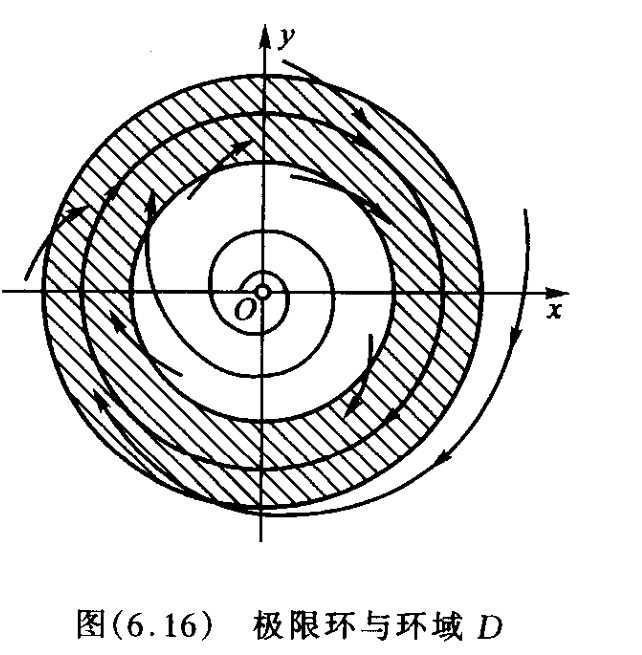
\includegraphics[width=\textwidth]{极限环.png}
    \caption{极限环}
    \label{fig:极限环}
\end{marginfigure}

假设平面驻定微分方程组
\begin{equation}\label{eq:6.33}
    \frac{\mathrm{d} x}{\mathrm{~d} t}=X(x, y), \quad \frac{\mathrm{d} y}{\mathrm{~d} t}=Y(x, y),
\end{equation}
其右端函数 $X, Y$ 在相平面的某域 $G$ 内有一阶连续偏导数。
\begin{theorem}
    如果 $G$ 内存在有界的环形闭域 $D$, 在其内不含有方程组 \eqref{eq:6.33} 的奇点,而 \eqref{eq:6.33} 的经过域 $D$ 上点的解 $x=x(t), y=$ $y(t)$ 当 $t \geqslant t_0$ (或 $t \leqslant t_0$ ) 时不离开该域, 则或者其本身是一个周期解(闭轨线),或者它按正向(或负向)趋近于 $D$ 内的某一周期解 (闭轨线).
\end{theorem}

\begin{theorem}[极限环的存在性]\label{theorem:limit_cycle_existence}
    如果于 $G$ 内存在单连通域 $D^*$, 在其内函数 $\frac{\partial X}{\partial x}+$ $\frac{\partial Y}{\partial y}$ 不变号且在 $D^*$ 内的任何子域上不恒等于零,则方程组 \eqref{eq:6.33} 在域 $D^*$ 内不存在任何周期解, 更不存在任何极限环.
\end{theorem}
\begin{proof}
    现在用反证法利用格林 (Green) 公式来证明定理. 假设 $D^*$ 内存在某周期为 $T$ 的周期解
    $$
        \Gamma: x=x(t), \quad y=y(t), \quad 0 \leqslant t \leqslant T,
    $$
    则对于由 $\Gamma$ 所围成的域 $D_{\Gamma}\left(\right.$ 显然 $\left.D_{\Gamma} \subset D^*\right)$ 有
    $$
        \begin{aligned}
              & \iint_{\mathrm{D}_{\Gamma}}\left(\frac{\partial X}{\partial x}+\frac{\partial Y}{\partial y}\right) \mathrm{d} x \mathrm{~d} y=\int_{\Gamma}(X \mathrm{~d} y-Y \mathrm{~d} x) \\
            = & \int_0^T\left(X \frac{\mathrm{~d} y}{\mathrm{~d} t}-Y \frac{\mathrm{~d} x}{\mathrm{~d} t}\right) \mathrm{d} t=\int_0^T(X Y-Y X) \mathrm{d} t=0,
        \end{aligned}
    $$
    这与定理的假设矛盾, 故在域 $D^*$ 内不存在任何周期解更不存在任何极限环。
\end{proof}

\section{奇点}

考虑二维(平面)一阶驻定微分方程组
\begin{equation}\label{eq:6.50}
    \begin{cases}
        \frac{\mathrm{d} x}{\mathrm{~d} t}=X(x, y), \\
        \frac{\mathrm{d} y}{\mathrm{~d} t}=Y(x, y),
    \end{cases}
\end{equation}
\begin{definition}[奇点]
    同时满足$X(x,y)=0$和$Y(x,y)=0$的点称为方程组的奇点。
\end{definition}
不妨设奇点为原点$(0,0)$,则$X(0,0)=Y(0,0)=0$。否则平移变换。

下面我们考虑驻定微分方程组是线性的情形下其轨线在相平面上的性态,并根据奇点邻域内轨线分布的不同性态来区分奇点的不同类型。这时方程的形式为
\begin{equation}\label{eq:6.51}
    \begin{cases}
        \frac{\mathrm{d} x}{\mathrm{~d} t}=a_{11}x+a_{12}y, \\
        \frac{\mathrm{d} y}{\mathrm{~d} t}=a_{21}x+a_{22}y,
    \end{cases}
\end{equation}
显然,坐标原点为奇点。如果方程组\ref{eq:6.51}的系数矩阵还满足
\[
    \begin{vmatrix}
        a_{11} & a_{12} \\
        a_{21} & a_{22}
    \end{vmatrix}\ne 0
\]
则此奇点还是唯一的。

根据线性代数的理论,我们知道,在线性变换下,奇点的类型是不变的,所以对于线性方程组\ref{eq:6.51},其奇点的类型与如下四种形式之一相同:
\[
    \left[\begin{array}{ll}\lambda & 0 \\ 0 & \mu\end{array}\right],\left[\begin{array}{ll}\lambda & 1 \\ 0 & \lambda\end{array}\right],\left[\begin{array}{ll}\lambda & 0 \\ 0 & \lambda\end{array}\right],\left[\begin{array}{rr}\alpha & \beta \\ -\beta & \alpha\end{array}\right]
\]
其中$\lambda,\mu,\alpha,\beta$为实数。这些标准形式是根据方程组\ref{eq:6.51}的特征方程来确定的。
\subsection{从特征根判断奇点类型}
\href{https://zhuanlan.zhihu.com/p/307458958}{见此文章总结}

奇点类型和特征根的关系如下:
\begin{table*}[ht!]
    \centering
    \begin{tabular}{ccc}
        \toprule
        奇点类型 & 特征根      & 稳定性条件            \\
        \midrule
        鞍点   & 实数异号     & 不稳定              \\
        结点   & 实数同号     & 实部为正时不稳定,实部为负时稳定 \\
        奇结点  & 重实数根     & 实部为正时不稳定,实部为负时稳定 \\
        焦点   & 复数,实部不为零 & 实部为正时不稳定,实部为负时稳定 \\
        中心   & 纯虚数      & 稳定,但不渐近稳定        \\
        \bottomrule
    \end{tabular}
    \caption{奇点类型、特征根与稳定性的关系}
    \label{tab:奇点类型与特征根的关系}
\end{table*}

\subsubsection{同号相异实根}
方程的标准类型为
$$\frac{\mathrm{d} \xi}{\mathrm{d} t}=\lambda_1 \xi, \frac{\mathrm{~d} \eta}{\mathrm{~d} t}=\lambda_2 \eta$$
相平面上的轨线形状如图\ref{fig:结点}所示。
\begin{figure}[h]
    \centering
    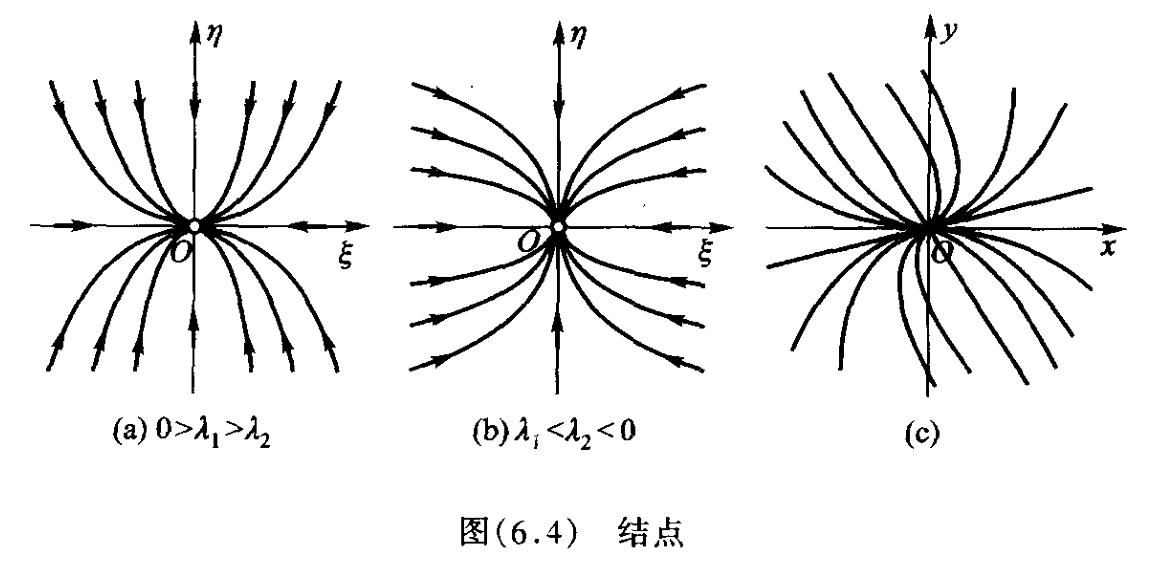
\includegraphics[width=\textwidth]{结点.png}
    \caption{结点}
    \label{fig:结点}
\end{figure}
图\ref{fig:结点}中,$\lambda_1,\lambda_2<0$,此时结点为\textbf{稳定结点},当$\lambda_1,\lambda_2>0$时,轨线走向相反。此时结点为\textbf{不稳定结点}。
\subsubsection{异号实根}

\begin{figure}[H]
    \centering
    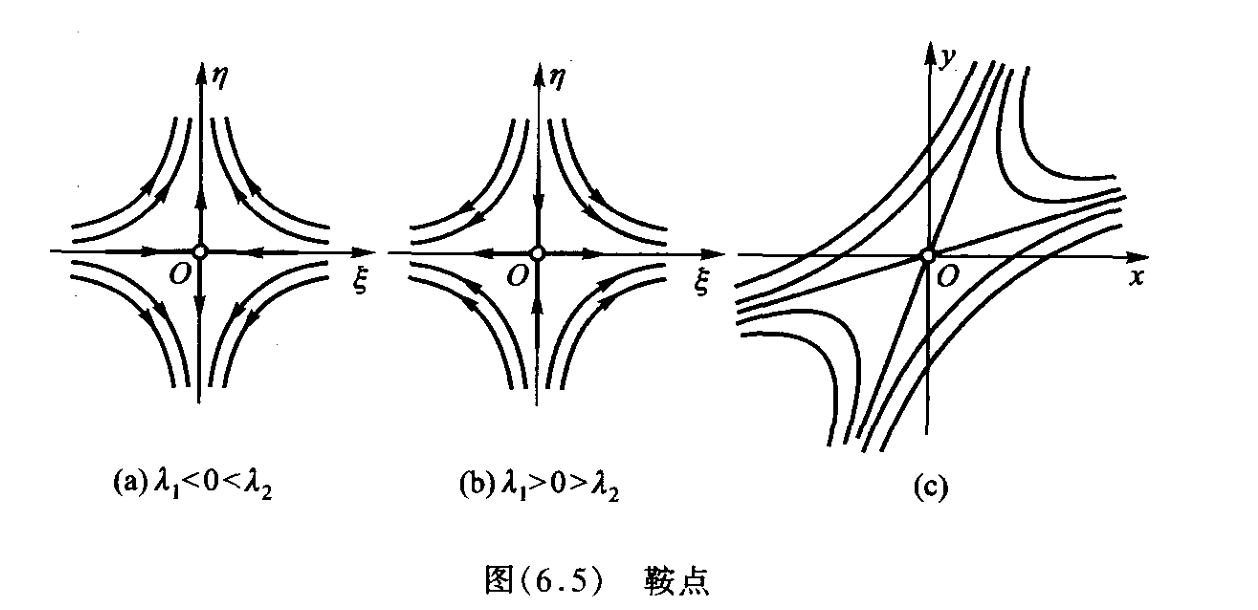
\includegraphics[width=\textwidth]{鞍点.png}
    \caption{鞍点}
    \label{fig:鞍点}
\end{figure}

\subsubsection{重根}
这时可以分两种情况讨论:

第一种是相似于
\[\left[\begin{array}{ll}\lambda & 1 \\ 0 & \lambda\end{array}\right]\]
方程可以化为
\[\frac{\mathrm{d} \xi}{\mathrm{d} t}=\lambda \xi+\eta, \quad \frac{\mathrm{d} \eta}{\mathrm{d} t}=\lambda \eta\]
其解为
\[
    \xi(t)=(At+B)\mathrm{e}^{\lambda t},\quad \eta(t)=A\mathrm{e}^{\lambda t}
\]
其中$\lambda$为实特征根,$A,B$为常数。
\begin{figure}[h]
    \centering
    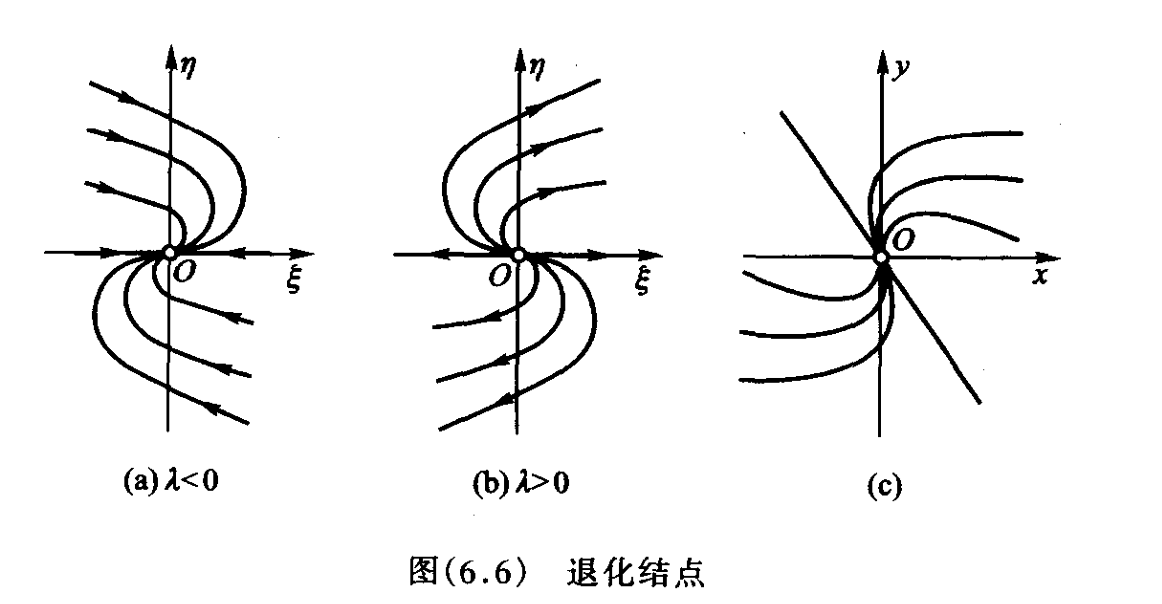
\includegraphics[width=\textwidth]{退化结点.png}
    \caption{退化结点}
    \label{fig:退化结点}
\end{figure}

第二种是相似于
\[\left[\begin{array}{ll}\lambda & 0 \\ 0 & \lambda\end{array}\right]\]
方程可以化为
\[\frac{\mathrm{d} x}{\mathrm{d} t}=\lambda x, \quad \frac{\mathrm{d} y}{\mathrm{d} t}=\lambda y\]
其解为
\[
    x(t)=A\mathrm{e}^{\lambda t},\quad y(t)=B\mathrm{e}^{\lambda t}
\]
其中$\lambda$为实特征根,$A,B$为常数。

于是
\[y=\frac{B}{A}x\]
\begin{figure}[h]
    \centering
    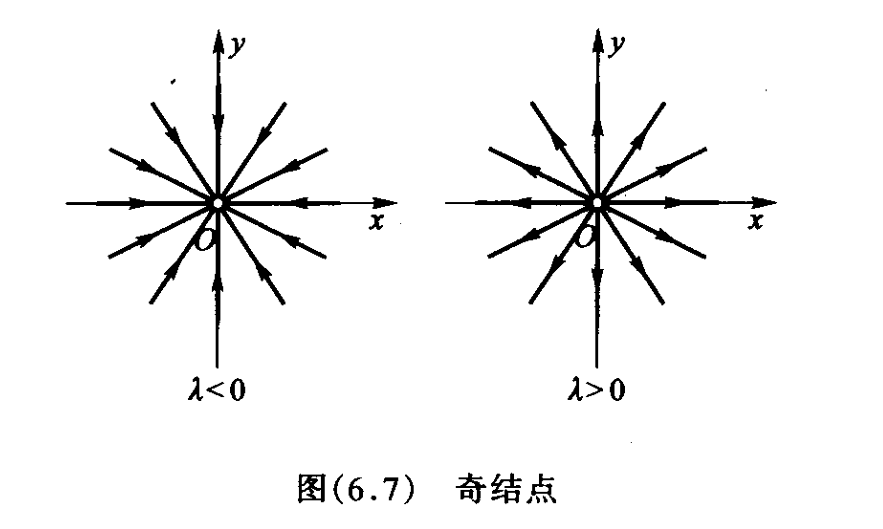
\includegraphics[width=\textwidth]{奇结点.png}
    \caption{奇结点}
    \label{fig:奇结点}
\end{figure}

\subsubsection{非零实部复根}
系数矩阵相似于
\[\left[\begin{array}{rr}\alpha & \beta \\ -\beta & \alpha\end{array}\right]\]
方程可以化为
\[\frac{\mathrm{d} \xi}{\mathrm{d} t}=\alpha \xi-\beta \eta, \quad \frac{\mathrm{d} \eta}{\mathrm{d} t}=\beta \xi+\alpha \eta\]
其解为
\[
    \xi(t)=A\mathrm{e}^{\alpha t}\cos(\beta t+\theta), \quad \eta(t)=A\mathrm{e}^{\alpha t}\sin(\beta t+\theta)
\]
其中$A,\theta$为常数。
\begin{figure}[h]
    \centering
    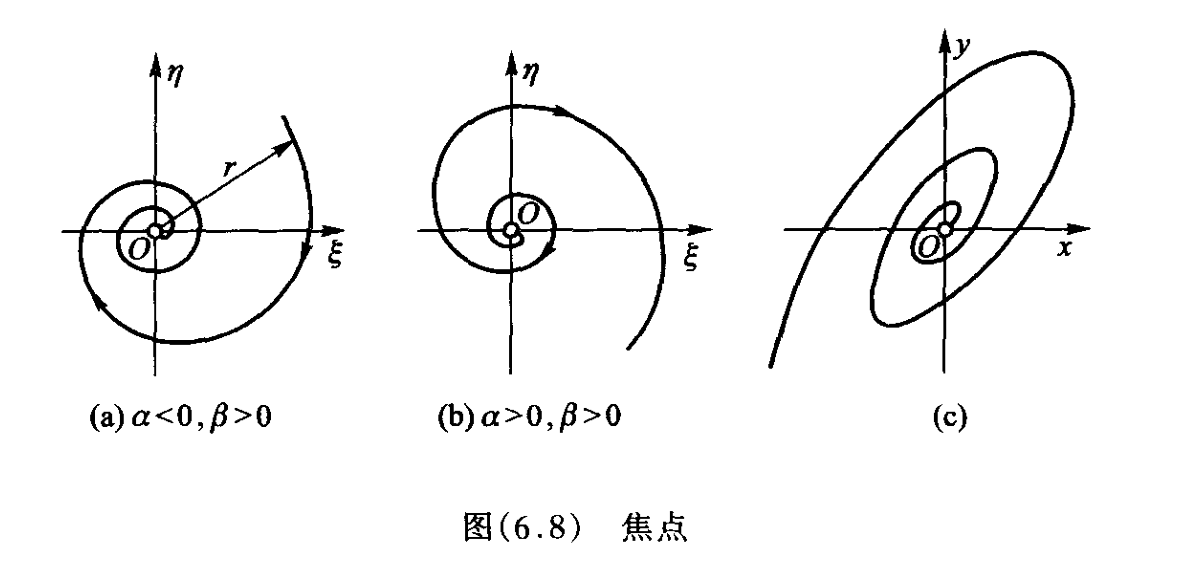
\includegraphics[width=\textwidth]{焦点.png}
    \caption{焦点}
    \label{fig:焦点}
\end{figure}

\subsubsection{纯虚根}
系数矩阵相似于\sidenote{也就是$\alpha=0$}
\[\left[\begin{array}{rr}0 & \beta \\ -\beta & 0\end{array}\right]\]
方程可以化为
\[\frac{\mathrm{d} x}{\mathrm{d} t}=-\beta y, \quad \frac{\mathrm{d} y}{\mathrm{d} t}=\beta x\]
其解为
\[
    x(t)=A\cos(\beta t+\theta), \quad y(t)=A\sin(\beta t+\theta)
\]
其中$A,\theta$为常数。
\begin{figure}[h]
    \centering
    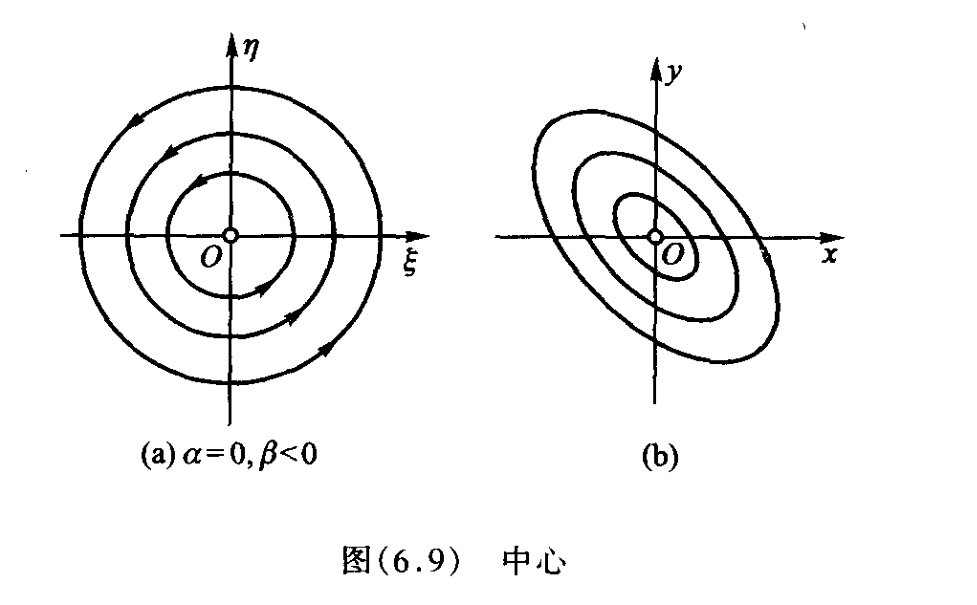
\includegraphics[width=\textwidth]{中心.png}
    \caption{中心}
    \label{fig:中心}
\end{figure}

\subsection{直接从特征方程判断奇点类型}
奇点的类型和特征方程的根之间的关系可以用图\ref{fig:奇点类型}来表示,对于特征方程
\[
    \lambda^2+p\lambda+q=0
\]
\begin{figure}[h]
    \centering
    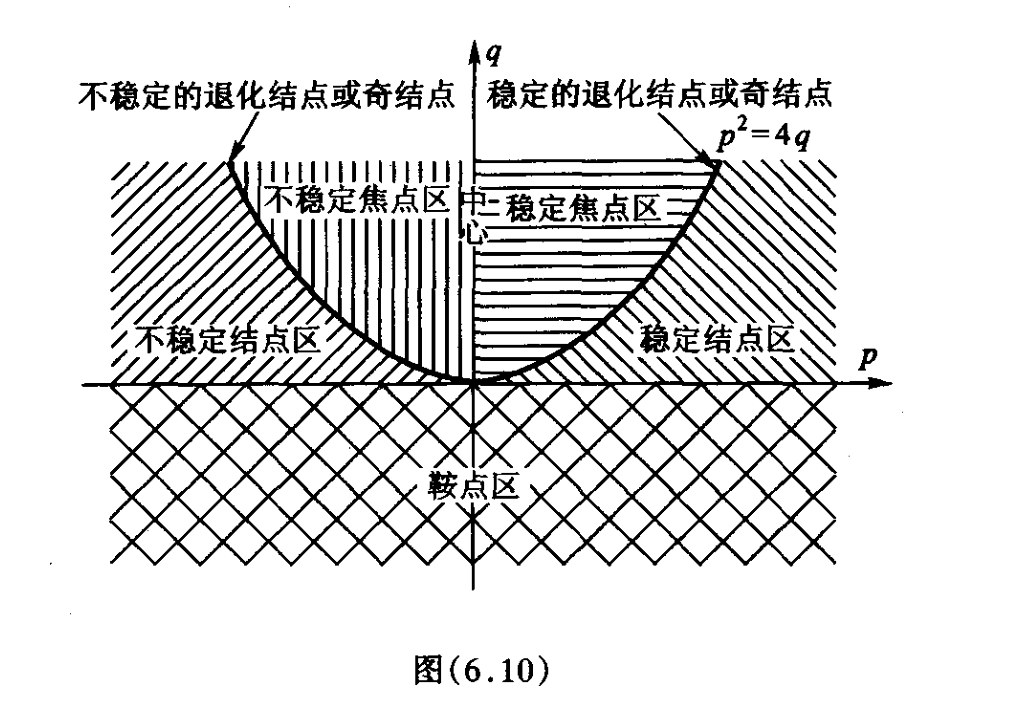
\includegraphics[width=\textwidth]{奇点类型.png}
    \caption{奇点类型}
    \label{fig:奇点类型}
\end{figure}

\section{练习}

\begin{exercise}
    $y^2(a d x-d y)-x(x+a y) d y=0$, 其中参数 $\mathrm{a}>0$;\marginnote{使用注意力}
\end{exercise}
\begin{remark}
    原方程可以变为齐次方程形式:$\frac{dy}{dx}=\frac{ay^2}{x^2+y^2+axy}$,但计算过程比较复杂。
\end{remark}
\begin{solution}
    注意到 $y\equiv 0$ 是特解: 若 $y\ne 0$ ,则原方程可变为: $\frac{y d x-x d y}{x^2+y^2}-\frac{1}{a y} d y=0$,因此通解为: $\arctan \frac{y}{x}-\frac{1}{a} \ln |y|=c$ 或 $y=x \tan \left(c+\frac{\ln |y|}{a}\right)$ ,其中, $c$ 是任意常数.
\end{solution}

\begin{exercise}
    $\frac{d}{d t}\binom{x}{y}=\left(\begin{array}{cc}-1 & 1 \\ 2 & 1\end{array}\right)\binom{x}{y}+\binom{e^{-t}}{0}$\marginnote{求解高阶微分方程,但是不使用特征根法}
\end{exercise}
\begin{remark}
    若用特征方法求解,容易出现计算错误。
\end{remark}
\begin{solution}
    由 $\left\{\begin{array}{c}x^{\prime}=-x+y+e^{-t} \\ y^{\prime}=2 x+y\end{array}\right.$ 得: $\left\{\begin{array}{l}y=x^{\prime}+x-e^{-t} \\ x^{\prime \prime}-3 x=-2 e^{-t}\end{array}\right.$

    现在求解方程: $\mathrm{x}^{\prime \prime}-3 \mathrm{x}=-2 e^{-t}$ 的通解为: $\mathrm{x}=c_1 e^{\sqrt{3} t}+c_2 e^{-\sqrt{3} t}+e^{-t}$

    最后, 原方程组的通解为:
    $\left\{\begin{array}{c}x=c_1 e^{\sqrt{3} t}+c_2 e^{-\sqrt{3} t}+e^{-t} \\ y=(1+\sqrt{3}) c_1 e^{\sqrt{3} t}+(1-\sqrt{3}) c_2 e^{-\sqrt{3} t}-e^{-t}\end{array}\right.$ ,其中 $c_1, c_2$ 为任意常数.
\end{solution}

\begin{exercise}
    对于一阶微分方程 $\frac{d y}{d x}=x^2-2 x y+y^2$,\marginnote{解的存在唯一性定理,Picard逐步逼近法,延拓解的存在区间,解对参数的偏导数}
    \begin{enumerate}
        \item 若 $-1 \leq x \leq 1,-1 \leq y \leq 1$, 试根据解的存在唯一性定理给出满足初始条件 $y(0)=0$ 的特解的存在区间;
        \item 若 $-1 \leq x \leq 1,-1 \leq y \leq 1$, 试根据Picard逐步逼近法给出满足初始条件 $y(0)=0$ 的二次近似解;
        \item 若 $-\infty \leq x \leq+\infty,-\infty \leq y \leq+\infty$, 试求满足初始条件 $y(0)=2$ 的延拓解的存在区间;
        \item 若 $-\infty \leq x \leq+\infty,-\infty \leq y \leq+\infty$ ,并记满足初始条件 $y\left(x_0\right)=y_0$ 的特解为 $\varphi\left(\mathrm{x} ; \mathrm{x}_0, \mathrm{y}_0\right)$, 试求偏导数函数: $\left.\frac{\partial \varphi\left(x ; x_0, y_0\right)}{\partial x_0}\right|_{x_0=0, y_0=1},\left.\frac{\partial \varphi\left(x ; x_0, y_0\right)}{\partial y_0}\right|_{x_0=0, y_0=1}$, $\left.\frac{\partial \varphi\left(x ; x_0, y_0\right)}{\partial x_0}\right|_{x_0=0, y_0=2},\left.\frac{\partial \varphi\left(x ; x_0, y_0\right)}{\partial y_0}\right|_{x_0=0, y_0=2}$ 的分析表达式.
    \end{enumerate}
\end{exercise}
\begin{solution}
    \begin{enumerate}
        \item 解: $f(x, y)=y^2-2 x y+x^2=(y-x)^2, a=1, b=1, M=\max |f(x, y)|=4$, $\mathrm{h}=\min \left(a, \frac{b}{M}\right)=\frac{1}{4}$. 因此, 解的存在区间为: $-\frac{1}{4} \leq x \leq \frac{1}{4}$
        \item 解: $x_0=0, \varphi_0(x)=y_0=0, \varphi_n(x)=y_0+\int_{x_0}^x f\left(s, \varphi_{n-1}(s)\right) d s, n=1,2, \ldots$

              一次近似解: $\varphi_1(x)=0+\int_0^x f\left(s, \varphi_0(s)\right) d s=\int_0^x(0-s)^2 d s=\frac{1}{3} x^3$
              二次近似解: $\varphi_2(x)=0+\int_0^x f\left(s, \varphi_1(s)\right) d s$
              $$
                  =\int_0^x\left(\frac{1}{3} s^3-s\right)^2 d s=\frac{1}{63} x^7-\frac{2}{15} x^5+\frac{1}{3} x^3
              $$
        \item 解: 对于 $\frac{d y}{d x}=(y-x)^2$, 令 $\mathrm{z}=\mathrm{y}-\mathrm{x}$, 则 $\frac{d z}{d x}=z^2-1=(z-1)(z+1)$,其通解为: $\mathrm{z}=\frac{1+c e^{2 x}}{1-c e^{2 x}}$, 其中 c 是任意常数, 因此 $\mathrm{y}=\mathrm{z}+\mathrm{x}=\frac{1+c e^{2 x}}{1-c e^{2 x}}+x$条件 $\mathrm{y}(0)=2$ 给出 $\mathrm{c}=\frac{1}{3}$, 因此满足 $\mathrm{y}(0)=2$ 的特解为: $\mathrm{y}=\frac{3+e^{2 x}}{3-e^{2 x}}+x$延拓解的存在区间为: $-\infty<x<\frac{1}{2} \ln 3$
    \end{enumerate}
\end{solution}

\begin{exercise}
    3. 设 $\boldsymbol{A}(t)$ 为区间 $a \leqslant t \leqslant b$ 上的连续 $n \times n$ 实矩阵, $\boldsymbol{\Phi}(t)$ 为方程 $\boldsymbol{x}'=$ $\boldsymbol{A}(t) \boldsymbol{x}$ 的基解矩阵,而 $\boldsymbol{x}=\boldsymbol{\varphi}(t)$ 为其一解。试证:
    \begin{enumerate}
        \item 对于方程 $\boldsymbol{y}'=-\boldsymbol{A}^{\mathrm{T}}(t) \boldsymbol{y}$ 的任一解 $\boldsymbol{y}=\boldsymbol{\psi}(t)$ 必有 $\boldsymbol{\psi}^{\mathrm{T}}(t) \boldsymbol{\varphi}(t)=$ 常数;
        \item $\boldsymbol{\Psi}(t)$ 为方程 $\boldsymbol{y}'=-\boldsymbol{A}^{\mathrm{T}}(t) \boldsymbol{y}$ 的基解矩阵的充要条件是存在非奇异的常数矩阵 $\boldsymbol{C}$, 使 $\boldsymbol{\Psi}^{\mathrm{T}}(t) \boldsymbol{\Phi}(t)=\boldsymbol{C}$.
    \end{enumerate}
\end{exercise}

\begin{proof}
    \begin{enumerate}
        \item 对于方程$\boldsymbol{y}'=-\boldsymbol{A}^{\mathrm{T}}(t) \boldsymbol{y}$,有$(y^\top)'=(y')^\top=(-A^\top y)^\top=-y^\top A$. 于是
              \[
                  \frac{d}{dt}(\boldsymbol{\psi}^\top \boldsymbol{\varphi})=(\boldsymbol{\psi}^\top)' \boldsymbol{\varphi}+\boldsymbol{\psi}^\top \boldsymbol{\varphi}'=-\boldsymbol{\psi}^\top A \boldsymbol{\varphi}+\boldsymbol{\psi}^\top A \boldsymbol{\varphi}=0
              \]
              于是$\boldsymbol{\psi}^\top \boldsymbol{\varphi}$为常数.
        \item 显然.
    \end{enumerate}
\end{proof}

\begin{exercise}
    $Y$是$\boldsymbol{x}'=\boldsymbol{A}(t)\boldsymbol{x}$的基解矩阵当且仅当$(Y^{-1})^{\top}$是$\boldsymbol{y}'=-\boldsymbol{A}^{\top}(t)\boldsymbol{y}$的一个基解矩阵.\sidenote{矩阵函数
        \[Q(t)=\begin{bmatrix}
                q_{11}(t) & q_{12}(t) & \cdots & q_{1n}(t) \\
                q_{21}(t) & q_{22}(t) & \cdots & q_{2n}(t) \\
                \vdots    & \vdots    & \ddots & \vdots    \\
                q_{n1}(t) & q_{n2}(t) & \cdots & q_{nn}(t)
            \end{bmatrix}
        \]
        被称为可微的,如果它的每个元素$q_{ij}(t)$都可微. 且$Q'(t)$被定义为
        \[
            Q'(t)=\begin{bmatrix}
                q_{11}'(t) & q_{12}'(t) & \cdots & q_{1n}'(t) \\
                q_{21}'(t) & q_{22}'(t) & \cdots & q_{2n}'(t) \\
                \vdots     & \vdots     & \ddots & \vdots     \\
                q_{n1}'(t) & q_{n2}'(t) & \cdots & q_{nn}'(t)
            \end{bmatrix}
        \]
    }
\end{exercise}

\begin{proof}
    对$Y^{-1}Y=I$两边求导,得到
    \[
        (Y^{-1}Y)'=Y^{-1}Y'+(Y^{-1})'Y=0
    \]
    于是$(Y^{-1}) ' Y=-Y^{-1}Y'=-Y^{-1}A(t)$. 由于$Y'=A(t)Y$,所以
    \[
        (Y^{-1})'=-Y^{-1}A(t)Y^{-1}=-Y^{-1}A(t)
    \]
    于是$((Y^{-1})^{\top})'=-A^{\top}(t)(Y^{-1})^{\top}$.
\end{proof}

\begin{exercise}
    求解 $x^{\prime \prime}(t)-9 x(t)=\mathrm{e}^{-3 t}\left(t^2+\sin 3 t\right)$.
\end{exercise}
\begin{solution}
    假设 $x(t)=\left(a t^3+b t^2+c t+m \cos 3 t+n \sin 3 t\right) \mathrm{e}^{-3 t}$, 则
    \[
        \frac{-18 a t^2+6 a t-12 b t+2 b-6 c+(18 m-9 n) \sin 3 t-(9 m+18 n) \cos 3 t}{\mathrm{e}^{3 t}}=\frac{t^2+\sin 3 t}{\mathrm{e}^{3 t}}
    \]
    解方程,得 $x_{\mathrm{p}}(t)=\frac{-180 t^3-90 t^2-30 t-72 \sin (3 t)+144 \cos (3 t)-5}{3240 \mathrm{e}^{3 t}}$ 为一特解。显然对应齐次方程的通解为 $x_{\mathrm{g}}(t)=c_1 \mathrm{e}^{3 t}+c_2 \mathrm{e}^{-3 t}$, 故所有解是
    \[
        x(t)=\frac{-180 t^3-90 t^2-30 t-72 \sin (3 t)+144 \cos (3 t)-5}{3240 \mathrm{e}^{3 t}}+c_1 \mathrm{e}^{3 t}+c_2 \mathrm{e}^{-3 t}
    \]
\end{solution}

\begin{exercise}
    考虑微分方程组: $\left\{\begin{array}{l}x^{\prime}=-x+y-x y^2 \\ y^{\prime}=-x-y-x^2 y\end{array}\right.$\marginnote{李雅普诺夫函数,极限环的存在性}
    \begin{enumerate}
        \item 试通过构造李雅谱洛夫函数,证明原点是渐近稳定的。(5 分)
        \item 试证明该系统在整个平面上无极限环。(5 分)
    \end{enumerate}
\end{exercise}

\begin{solution}
    \begin{enumerate}
        \item 构造李雅普诺夫函数$V(x,y)=x^2+y^2$,则
              \[
                  \frac{dV}{dt}=\frac{\partial V}{\partial x}\frac{dx}{dt}+\frac{\partial V}{\partial y}\frac{dy}{dt}=-2x^2-2y^2-4x^2y^2<0\quad(x,y)\ne (0,0)
              \]
              因此原点是渐近稳定的。
        \item 利用定理\ref{theorem:limit_cycle_existence},只需证明$\frac{\partial X}{\partial x}+\frac{\partial Y}{\partial y}$在平面上不变号且在平面上不为零。
              \[
                  \frac{\partial X}{\partial x}+\frac{\partial Y}{\partial y}=-1-1-x^2-y^2<0
              \]
              因此该系统在整个平面上无极限环。
    \end{enumerate}
\end{solution}

\begin{exercise}
    五. (20 分) 求出下列平面系统的所有奇点, 并判断奇点在相应线性近似方程中的类型:\marginnote{求解奇点并判断类型}
    $$
        \left\{\begin{array}{l}
            \frac{d x}{d t}=x^2-4 y \\
            \frac{d y}{d t}=x^2-(y-3)^2
        \end{array}\right.
    $$
\end{exercise}

\begin{solution}
    $$
        \left\{\begin{aligned}
            x^2-4 y     & =0 \\
            x^2-(y-3)^2 & =0
        \end{aligned}\right.
    $$
    $\Rightarrow(2,1),(-2,1),(6,9),(-6,9)$ 为所有奇点.
    $\left(x_0, y_0\right)$ 处线性近似对应矩阵
    $$
        \begin{gathered}
            A\left(x_0, y_0\right)=\left.\left(\begin{array}{ll}
                    2 x & -4      \\
                    2 x & -2(y-3)
                \end{array}\right)\right|_{\left(x_0, y_0\right)} \\
            A(2,1)=\left(\begin{array}{ll}
                    4 & -4 \\
                    4 & 4
                \end{array}\right) \\
            \operatorname{det}(A(2,1)-\lambda I)=\lambda^2-8 \lambda+32=(\lambda-4-4 i)(\lambda-4+4 i)
        \end{gathered}
    $$
    特征值为具有正实部的复数, $(2,1)$ 为(不稳定)焦点。
    同理可以知道 $A(-2,1)$ 特征值为 $\pm 4 \sqrt{2}$ 异号实数, $(-2,1)$ 为鞍点; $A(6,9)$ 特征值为 $\pm 4 \sqrt{6}$ 异号实数, $(6,9)$ 为鞍点; $A(-6,9)$ 特征值为 $-12 \pm 4 \sqrt{3}$ 为同号相异实数且同为负数, $(-2,1)$ 为稳定结点.
\end{solution}

\begin{exercise}
    12.已知方程组
    $$
        \left\{\begin{array}{l}
            \frac{\mathrm{d} x_1}{\mathrm{~d} t}=\frac{1}{t} x_1-x_2+t, \\
            \frac{\mathrm{~d} x_2}{\mathrm{~d} t}=\frac{1}{t^2} x_1+\frac{2}{t} x_2-t^2,
        \end{array} \quad t>0\right.
    $$
    的对应齐次方程组有解 $x_1=t^2, x_2=-t$ ,求其通解.
\end{exercise}
\begin{solution}
    由定理\ref{thm:4.8},设对应的齐次方程有另一解$y_1,y_2$,则
    $$
        \begin{vmatrix}
            t^2 & y_1 \\
            -t & y_2
        \end{vmatrix}=\exp\left(\int\frac{1}{t}+\frac{2}{t}dt\right)=t^3
    $$
    也就是$y_1=t^2-ty_2$,带入齐次方程组的第2个方程得到$\frac{dy_2}{dt}=t^{-1}y_2+1$,解得$y_2=t\ln t$,从而$y_1=t^2-t^2\ln t$,于是有基解矩阵
    \[
        \Phi(t)=\begin{bmatrix}
            t^2 & t^2(1-\ln t) \\
            -t & t\ln t
        \end{bmatrix}
    \]
    现在利用常数变易法求解非线性方程组的一个特解,只需照章办事,就有
    $$
        \tilde{x}=\begin{bmatrix}
            \frac{t^2}{2}\ln t-\frac{t^2}{2}(\ln t)^2+\frac{t^4}{4}-\frac{t^2}{4} \\
            \frac{t}{2}(\ln t)^2+\frac{t}{2}\ln t -\frac{3}{4}t^3+\frac{3}{4}t
        \end{bmatrix}
    $$
    于是通解为
    \[
        x=t^2\begin{bmatrix}
            t^2 & t^2(1-\ln t) \\
            -t & t\ln t
        \end{bmatrix}\begin{bmatrix}c_1 \\ c_2\end{bmatrix}+\begin{bmatrix}
            \frac{t^2}{2}\ln t-\frac{t^2}{2}(\ln t)^2+\frac{t^4}{4}-\frac{t^2}{4} \\
            \frac{t}{2}(\ln t)^2+\frac{t}{2}\ln t -\frac{3}{4}t^3+\frac{3}{4}t
        \end{bmatrix}
    \]
\end{solution}



\begin{thebibliography}{99}
    \bibitem{王高雄} 王高雄, 周之铭, 朱思铭, 王寿松. 常微分方程[M]. 第三版. 高等教育出版社, 2006.
    \bibitem{张伟年} 张伟年, 杜正东, 徐冰. 常微分方程[M]. 第二版. 高等教育出版社, 2014.
    \bibitem{Trench} William F. Trench. Elementary Differential Equations. 2013.
    \bibitem{Arnold} V.I.Arnold. Ordinary Differential Equations. 2010.
    \bibitem{Walter} Wolfgang Walter. Ordinary Differential Equations. Graduate Texts in Mathematics, Vol. 182. Springer-Verlag, 1998.
\end{thebibliography}

